\documentclass[
	12pt,				% Tamanho da fonte
	oneside,			% Para impressão apenas no anverso (apenas frente). Oposto a twoside
	a4paper,			% Tamanho do papel
	english,			% Idioma adicional para hifenização
	brazil				% O último idioma é o principal do documento
]{abntex2}

% Pacotes básicos
\usepackage[utf8]{inputenc}			% Codificação do documento (conversão automática dos acentos)
\usepackage{lastpage}				% Usado pela Ficha catalográfica
\usepackage{indentfirst}			% Indenta o primeiro parágrafo de cada seção
\usepackage{color}					% Controle das cores
\usepackage{graphicx}				% Inclusão de gráficos
\usepackage{microtype} 				% Melhorias de justificação
\usepackage{pdfpages}     			% Incluir PDFs
\usepackage{algorithm}				% Ilustrações do tipo algoritmo
\usepackage{mdwlist}				% Itens com espaço padrão da abnt
\usepackage[noend]{algpseudocode}	% Ilustrações do tipo algoritmo
		
% Pacotes adicionais
\usepackage{lipsum}					% Geração de dummy text
\usepackage{bigstrut}
\usepackage[table]{xcolor}
\usepackage{tabularx}

% Pacotes de citações
\usepackage[brazilian,hyperpageref]{backref}	 					% Paginas com as citações na bibl
\usepackage[alf,abnt-etal-list=0,abnt-etal-text=it]{abntex2cite}	% Citações padrão ABNT

% Configuração de pacotes
\graphicspath{{images/}} 									% Diretório padrão de imagens
\renewcommand{\backrefpagesname}{Citado na(s) página(s):~}	% Configurações do pacote backref - Usado sem a opção hyperpageref de backref
\renewcommand{\backref}{} 									% Texto padrão antes do número das páginas
\renewcommand*{\backrefalt}[4]{ 							% Define os textos da citação
	\ifcase #1 Nenhuma citação no texto.
	\or Citado na página #2.
	\else Citado #1 vezes nas páginas #2.
	\fi
}






























% Informações de dados para capa e folha de rosto
\instituicao{
	UNIVERSIDADE DE SÃO PAULO
	\par
	PROGRAMA DE PÓS-GRADUAÇÃO EM ENGENHARIA MECÂNICA
}
\titulo{Integração da memória digital de produtos ao RAMI4.0 para monitoramento de itens ao longo da cadeia de valor}
\autor{\uppercase{Henrique Abrantes Vitoi}}
\local{São Paulo}
\data{2020}
\orientador{Prof. Dr. Fabrício Junqueira}
\coorientador{Prof. Dr. Paulo Eigi Miyagi}
\tipotrabalho{Dissertação (Mestrado)}

\preambulo{
	Versão original
	\newline \newline \newline
	Dissertação apresentada à Escola Politécnica da Universidade de São Paulo para obtenção do título de Mestre em Ciências pelo Programa de Pós-graduação em Engenharia Mecânica. 
	\newline \newline
	Área de concentração: Engenharia de Controle e Automação Mecânica
	\newline \newline \newline
	Versão corrigida contendo as alterações solicitadas pela comissão julgadora em \_\_\_\_\_\_\_ de \_\_\_\_\_\_\_\_\_\_\_\_\_\_\_\_\_\_\_\_\_\_ de \_\_\_\_\_\_\_\_\_\_. A versão original encontra-se em acervo reservado na Biblioteca da POLI-USP e na Biblioteca Digital de Teses e Dissertações da USP (BDTD), de acordo com a Resolução CoPGr 6018, de 13 de outubro de 2011.
}

\definecolor{blue}{RGB}{41,5,195}	% Altera o aspecto da cor azul

% Informações do PDF
\makeatletter
\hypersetup{
     	%pagebackref=true,
		pdftitle={\@title}, 
		pdfauthor={\@author},
    	pdfsubject={\imprimirpreambulo},
	    pdfcreator={LaTeX com abnTeX2 adaptado para o PPGEM-POLI-USP},
		pdfkeywords={abnt}{latex}{abntex}{abntex2}{qualificação de mestrado}{dissertação de mestrado}{ppgsi}, 
		colorlinks=true,       		% false: boxed links; true: colored links
    	linkcolor=black,          	% color of internal links
    	citecolor=black,        	% color of links to bibliography
    	filecolor=black,      		% color of file links
		urlcolor=black,
		bookmarksdepth=4
}
\makeatother

% Tamanho do parágrafo
\setlength{\parindent}{1.25cm}

% Espaçamento entre parágrafos
\setlength{\parskip}{0cm}  % Tente também \onelineskip
\renewcommand{\baselinestretch}{1.5}
\makeindex % Compila o índice

% Controlar linhas órfãs e viúvas
\clubpenalty10000
\widowpenalty10000
\displaywidowpenalty10000
























% ----------------------------------------------------------
% ELEMENTOS PRÉ-TEXTUAIS
% ----------------------------------------------------------
\begin{document}
\frenchspacing 		% Retira espaço extra obsoleto entre as frases
\imprimircapa
\imprimirfolhaderosto*

\begin{fichacatalografica}
    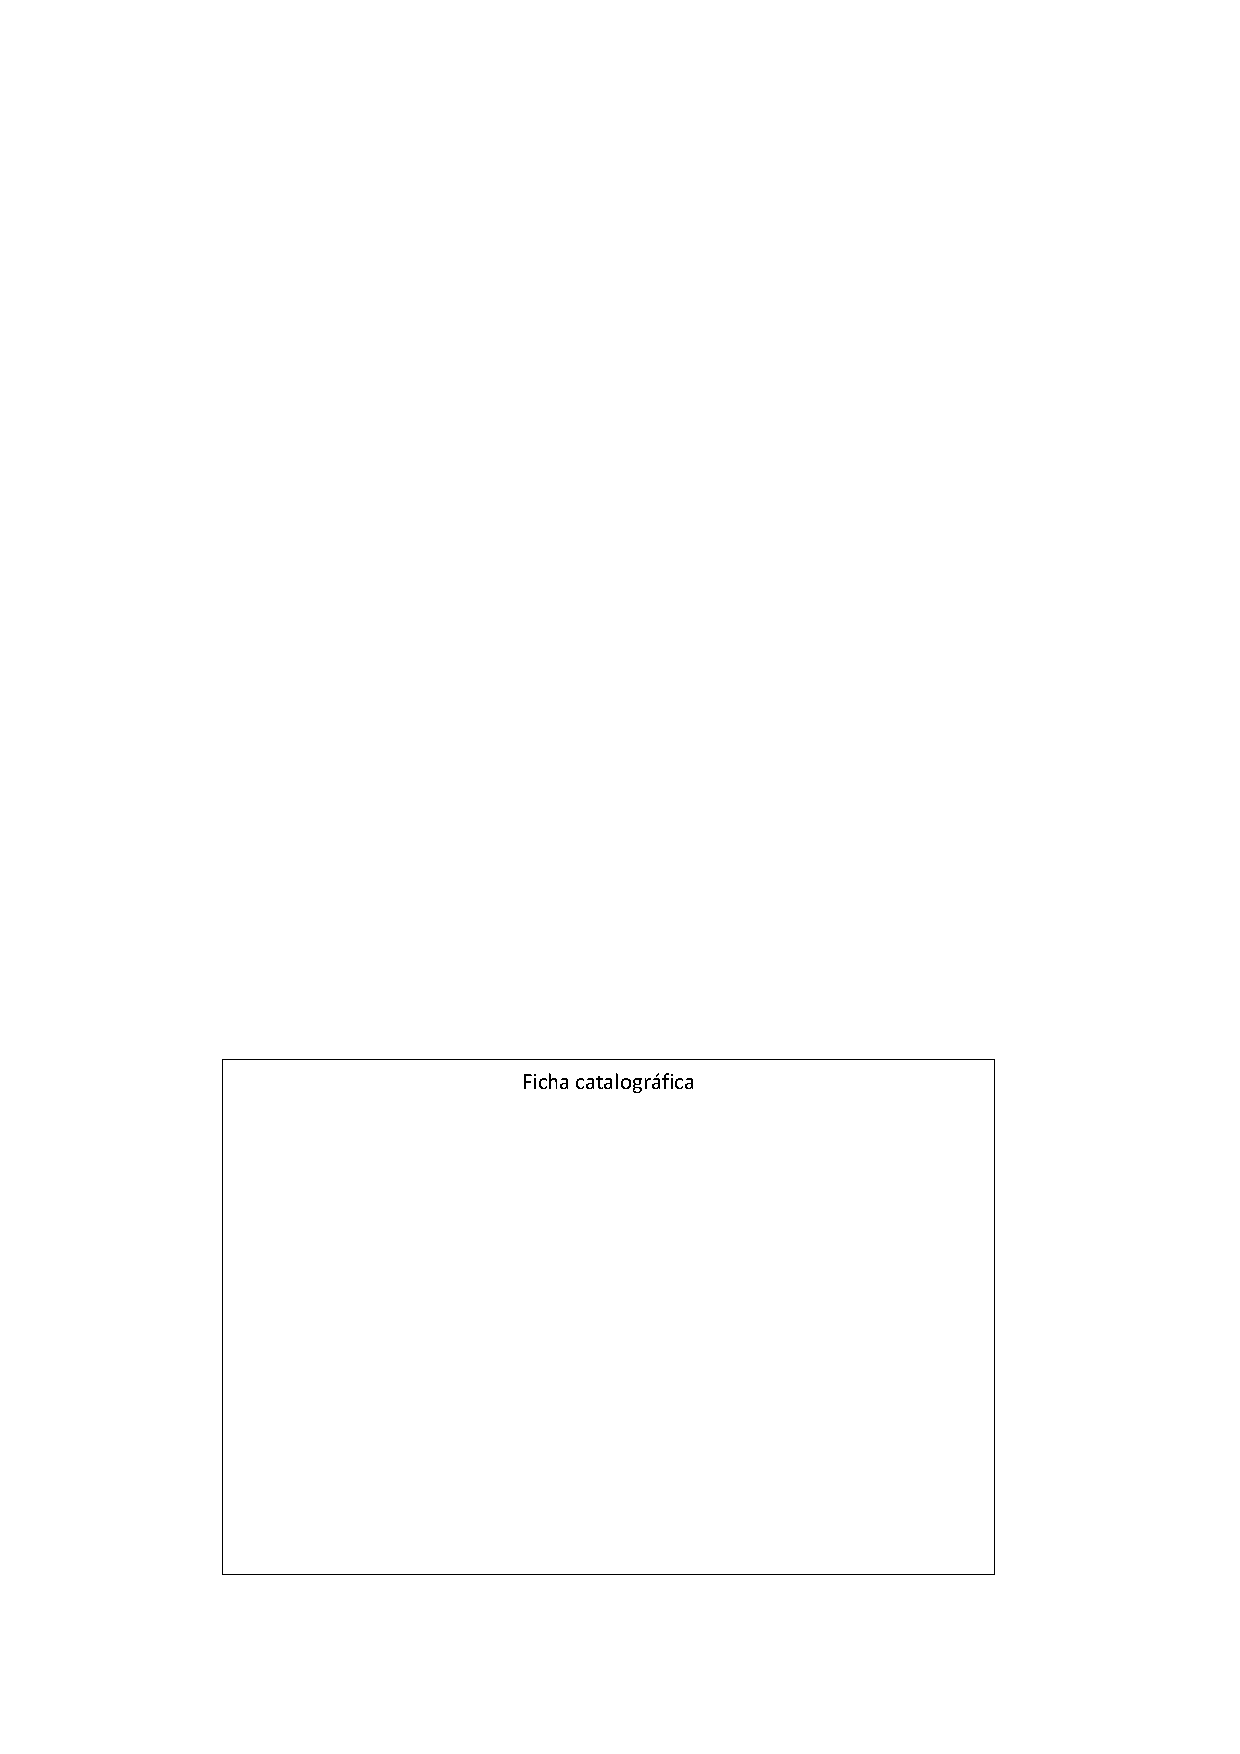
\includepdf{ficha_catalografica.pdf}
\end{fichacatalografica}

\begin{folhadeaprovacao}

	\noindent Dissertação de autoria de Henrique Abrantes Vitoi, sob o título \textbf{``\imprimirtitulo''}, apresentada à Escola Politécnica da Universidade de São Paulo, para obtenção do título de Mestre em Ciências pelo Programa de Pós-graduação em Engenharia Mecânica, na área de concentração Engenharia de Controle e Automação Mecânica, aprovada em \_\_\_\_\_\_\_ de \_\_\_\_\_\_\_\_\_\_\_\_\_\_\_\_\_\_\_\_\_\_ de \_\_\_\_\_\_\_\_\_\_ pela comissão julgadora constituída pelos doutores:
	\vspace*{3cm}
	\begin{center}
		\_\_\_\_\_\_\_\_\_\_\_\_\_\_\_\_\_\_\_\_\_\_\_\_\_\_\_\_\_\_\_\_\_\_\_\_\_\_\_\_\_\_\_\_\_\_\_\_\_\_\_\_\_\_\_\_
		\vspace*{0.2cm} 
		\\ \textbf{Prof. Dr. \_\_\_\_\_\_\_\_\_\_\_\_\_\_\_\_\_\_\_\_\_\_\_\_\_\_\_\_\_\_\_\_\_\_\_\_\_\_\_\_\_\_\_\_\_\_\_\_\_\_\_\_\_\_\_\_\_\_\_\_\_\_} 
		\\ \vspace*{0.2cm} 
		Instituição: \_\_\_\_\_\_\_\_\_\_\_\_\_\_\_\_\_\_\_\_\_\_\_\_\_\_\_\_\_\_\_\_\_\_\_\_\_\_\_\_\_\_\_\_\_\_\_\_\_\_\_\_\_\_\_\_\_\_ 
		\\ \vspace*{0.2cm}
		Presidente 

		\vspace*{2cm}

		\_\_\_\_\_\_\_\_\_\_\_\_\_\_\_\_\_\_\_\_\_\_\_\_\_\_\_\_\_\_\_\_\_\_\_\_\_\_\_\_\_\_\_\_\_\_\_\_\_\_\_\_\_\_\_\_
		\vspace*{0.2cm} 
		\\ \textbf{Prof. Dr. \_\_\_\_\_\_\_\_\_\_\_\_\_\_\_\_\_\_\_\_\_\_\_\_\_\_\_\_\_\_\_\_\_\_\_\_\_\_\_\_\_\_\_\_\_\_\_\_\_\_\_\_\_\_\_\_\_\_\_\_\_\_} 
		\\ \vspace*{0.2cm} 
		Instituição: \_\_\_\_\_\_\_\_\_\_\_\_\_\_\_\_\_\_\_\_\_\_\_\_\_\_\_\_\_\_\_\_\_\_\_\_\_\_\_\_\_\_\_\_\_\_\_\_\_\_\_\_\_\_\_\_\_\_

		\vspace*{2cm}

		\_\_\_\_\_\_\_\_\_\_\_\_\_\_\_\_\_\_\_\_\_\_\_\_\_\_\_\_\_\_\_\_\_\_\_\_\_\_\_\_\_\_\_\_\_\_\_\_\_\_\_\_\_\_\_\_
		\vspace*{0.2cm} 
		\\ \textbf{Prof. Dr. \_\_\_\_\_\_\_\_\_\_\_\_\_\_\_\_\_\_\_\_\_\_\_\_\_\_\_\_\_\_\_\_\_\_\_\_\_\_\_\_\_\_\_\_\_\_\_\_\_\_\_\_\_\_\_\_\_\_\_\_\_\_} 
		\\ \vspace*{0.2cm} 
		Instituição: \_\_\_\_\_\_\_\_\_\_\_\_\_\_\_\_\_\_\_\_\_\_\_\_\_\_\_\_\_\_\_\_\_\_\_\_\_\_\_\_\_\_\_\_\_\_\_\_\_\_\_\_\_\_\_\_\_\_

		\vspace*{2cm}

		\_\_\_\_\_\_\_\_\_\_\_\_\_\_\_\_\_\_\_\_\_\_\_\_\_\_\_\_\_\_\_\_\_\_\_\_\_\_\_\_\_\_\_\_\_\_\_\_\_\_\_\_\_\_\_\_
		\vspace*{0.2cm} 
		\\ \textbf{Prof. Dr. \_\_\_\_\_\_\_\_\_\_\_\_\_\_\_\_\_\_\_\_\_\_\_\_\_\_\_\_\_\_\_\_\_\_\_\_\_\_\_\_\_\_\_\_\_\_\_\_\_\_\_\_\_\_\_\_\_\_\_\_\_\_} 
		\\ \vspace*{0.2cm} 
		Instituição: \_\_\_\_\_\_\_\_\_\_\_\_\_\_\_\_\_\_\_\_\_\_\_\_\_\_\_\_\_\_\_\_\_\_\_\_\_\_\_\_\_\_\_\_\_\_\_\_\_\_\_\_\_\_\_\_\_\_
	\end{center}
  
\end{folhadeaprovacao}

% Resumo em português
\setlength{\absparsep}{18pt}	% Ajusta o espaçamento dos parágrafos
\begin{resumo}

	\begin{flushleft}
		VITOI, Henrique Abrantes. \textbf{Título do trabalho}: \imprimirtitulo. \imprimirdata. \pageref{LastPage} f. Dissertação (Mestrado em Ciências) – Escola Politécnica, Universidade de São Paulo, São Paulo, 2020.
	\end{flushleft}

	A mudança de paradigma na indústria referente às recentes modificações em relação às tecnologias de manufatura é chamada de Indústria 4.0. Nesse novo conceito, redes inteligentes de máquinas e processos para indústria com o respaldo de tecnologias da informação e comunicação passam a proporcionar um alto nível de automação e intercâmbio de informações entre equipamentos, produtos e demais atores em um ambiente de manufatura.
	Este trabalho aborda uma proposta de desenvolvimento dos detalhes do Modelo de Arquitetura de Referência para a Indústria 4.0 (RAMI4.0), especificamente por meio da introdução do conceito de Memória Digital do Produto (MDP) ao eixo horizontal ``Ciclo de Vida e Cadeia de Valor'', de forma a se aperfeiçoar a elaboração dessa arquitetura a fim de proporcionar mais robustez ao modelo para uma futura adoção generalizada por parte de empresas por todo o mundo.
	O estudo é feito com o objetivo de aperfeiçoar o RAMI4.0 no sentido de propiciar o surgimento de novos cenários de criação de valor no contexto de Indústria 4.0 (I4.0) e incentivar a geração de novos modelos de negócio baseado em dados.

	Palavras-chaves: Indústria 4.0. RAMI4.0. Memória digital do produto. Cadeia de Valor. Ciclo de vida do produto.
	
\end{resumo}

% Resumo em inglês
\begin{resumo}[Abstract]
	\begin{otherlanguage*}{english}

		\begin{flushleft}
			VITOI, Henrique Abrantes. \textbf{Work title}: work subtitle. \imprimirdata. \pageref{LastPage} p. Dissertation (Master of Science) – School of Arts, Sciences and Humanities, University of São Paulo, São Paulo, DefenseYear. 
		\end{flushleft}
		Abstract here

		Keywords: Industry 4.0. RAMI4.0. Digital product memory. Value Chain. Product life cycle. 
	\end{otherlanguage*}
\end{resumo}

% Inserir lista de figuras
\pdfbookmark[0]{\listfigurename}{lof}
\listoffigures*
\cleardoublepage

% Inserir lista de algoritmos
%\pdfbookmark[0]{\listalgorithmname}{loa}
%\listofalgorithms
%\cleardoublepage

% Inserir lista de quadros
%\pdfbookmark[0]{\listofquadrosname}{loq}
%\listofquadros*
%\cleardoublepage

% Inserir lista de tabelas
\pdfbookmark[0]{\listtablename}{lot}
\listoftables*
\cleardoublepage

% Inserir lista de abreviaturas e siglas
\begin{siglas}
	\item[AAS] \textit{Asset Administration Shell} (Camada Administrativa do Ativo)
	\item[CS] Cadeia de Suprimentos
	\item[CV] Cadeia de Valor
	\item[CVP] Ciclo de Vida do Produto
	\item[GCVP] Gestão do Ciclo de Vida do Produto
	\item[I4.0] Indústria 4.0
	\item[IIoT] \textit{Industrial Internet of Things} (Internet das Coisas Industrial)
	\item[IoT] \textit{Internet of Things} (Internet das Coisas)
	\item[MDP] Memória Digital do Produto
	\item[RAMI4.0] \textit{Reference Architectural Model Industrie 4.0} (Modelo de Arquitetura de Referência para a Indústria 4.0)
  	\item[TIC] Tecnologia da Informação e Comunicação
  	
  	
  	
\end{siglas}

% Inserir lista de símbolos
%\begin{simbolos}
%  \item[$ \in $] Pertence
%\end{simbolos}

% Inserir Sumário
\pdfbookmark[0]{\contentsname}{toc}
\tableofcontents*
\cleardoublepage
































% ----------------------------------------------------------
% ELEMENTOS TEXTUAIS
% ----------------------------------------------------------
\textual

\chapter{Introdução}

	O cenário atual de comércio em um mundo intrinsecamente globalizado requer eficiência em troca de informações, serviços e mercadorias; ou seja, eficiência logística. A logística é a essência do comércio \cite{ballou2006cadeiasuprimentos}, ela contribui para que pessoas não mais sejam obrigadas a viver perto das fontes de produção e possam trocar mercadorias com outras regiões de forma efetiva, contribuindo decisivamente para melhorar o padrão econômico de vida geral. 
	
	A logística é o processo de planejamento, implantação e controle do fluxo eficiente e eficaz de mercadorias, serviços e das informações relativas desde o ponto de origem até o ponto de consumo com o propósito de atender as exigências dos clientes \cite{cscmp2013supplychainglossary}. Essa definição sugere a logística como um processo, o que significa que inclui todas as atividades importantes para a disponibilização de bens e serviços aos consumidores quando e onde estes quiserem adquiri-los \cite{ballou2006cadeiasuprimentos}.
	
	A cadeia de suprimentos (CS), por outro lado, é um conceito mais amplo. A CS é onde a logística é exercida. São as partes necessárias para se dar suporte ao pedido de um cliente, desde o produtor até o consumidor final. A gestão da cadeia de suprimentos tem como alvo a orquestração de todas as partes envolvidas por meio de uma logística integrada de forma a se otimizar ao máximo o processo de fornecimento de um produto, serviço ou informação.
	
	A ideia de uma CS simples envolve fornecedor, produtor e cliente \cite{hugos2018supplychain}, porém conceitos modernos ampliam a noção de CS para uma cadeia de suprimentos estendida, que inclui diversos outros fornecedores de serviços em áreas como logística, finanças, \textit{marketing} e desenvolvimento; que, mediante coordenação e colaboração, criam oportunidades para melhoria dos custos ou serviços ao consumidor. A Figura \ref{fig:cadeia-de-suprimentos} exemplifica a inter-relação das partes em uma cadeia de suprimentos estendida.
	
	\begin{figure}[H]
		\centering
		\caption{Exemplo de cadeia de suprimentos estendida.}
		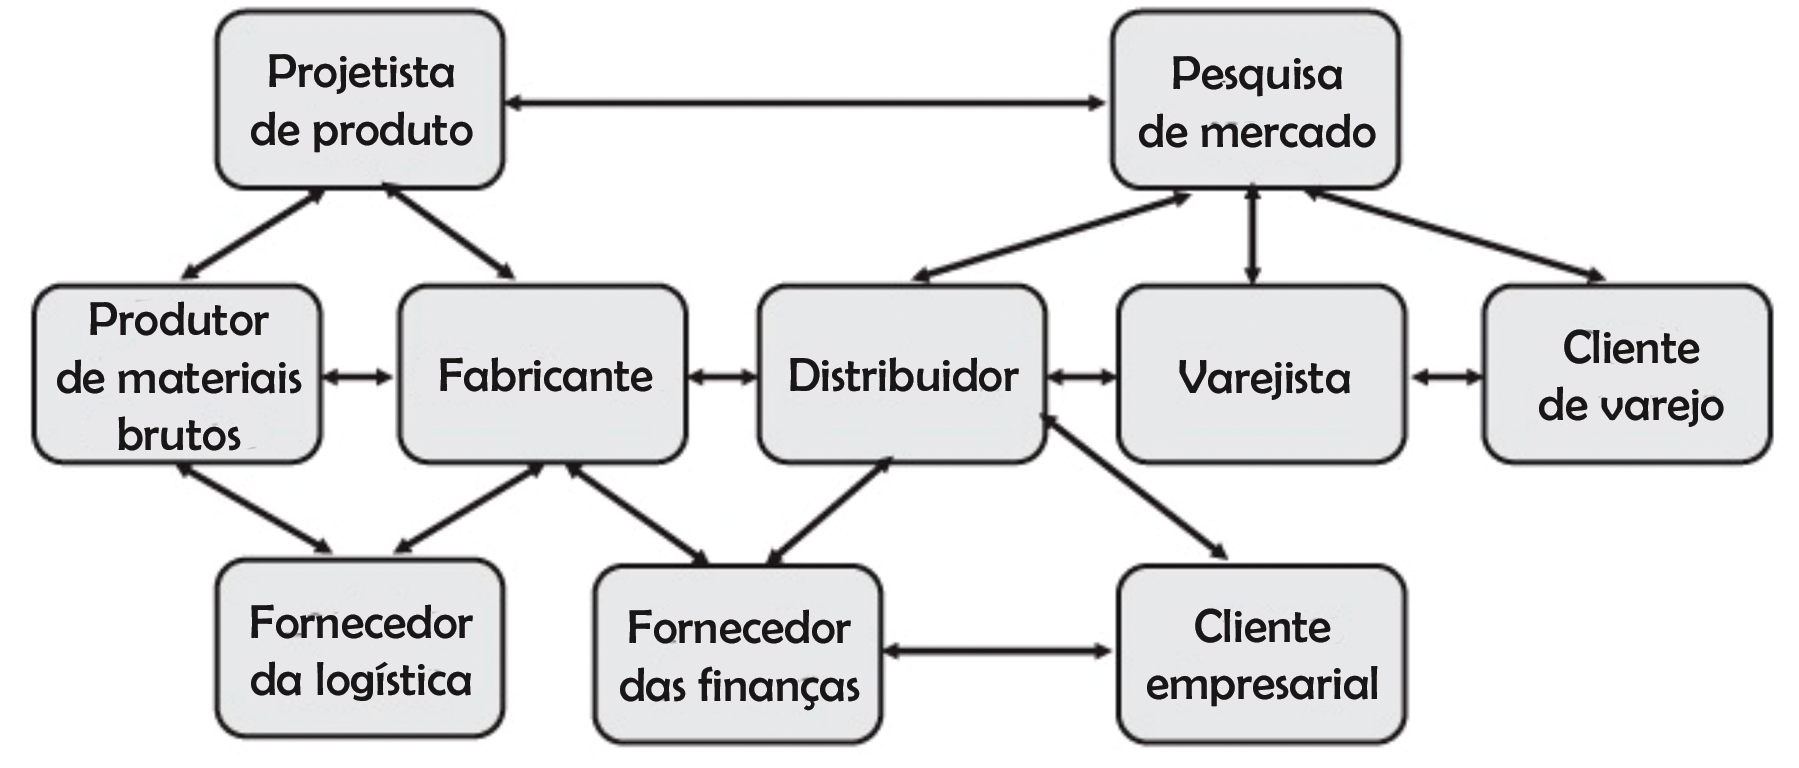
\includegraphics[width=1\textwidth]{cadeia-de-suprimentos.png}
		\label{fig:cadeia-de-suprimentos}
		\source{\citeonline{hugos2018supplychain} (adaptado).}
	\end{figure}

	Além do eficiente fluxo de materiais e produtos dentro da CS, é imprescindível a manutenção de um canal para troca de informações entre as partes em uma CS, pois sem uma adequada comunicação, gerentes podem acidentalmente tomar decisões supostamente racionais, porém que afetam negativamente outros líderes da cadeia, como o efeito chicote \cite{lee1997bullwhip}, que é a distorção da percepção da procura de um produto que vai se ampliando ao longo da cadeia de suprimentos. Erros de comunicação desse tipo podem acarretar problemas como o aumento do custo de transporte, o elevado tempo de aprovisionamento ao cliente e o desgaste no relacionamento com os fornecedores.
	
	Ao longo da cadeia de suprimentos pode-se observar processos que agregam valor ao produto em desenvolvimento. As etapas de transformação do produto com adição de valor ao longo da CS também podem ser definidas como cadeia de valor.
	
	Uma cadeia de valor (CV) é um conjunto de atividades que empresas de um setor específico desempenham a fim de entregar um produto ou serviço que tenha algum valor perceptível para o mercado \cite{porter1985competitiveadvantage}. A ideia da CV é baseada na agregação de valor ao produto a cada processo de transformação ocorrido, processo esse que envolve a aquisição e consumo de recursos (mão de obra, materiais, equipamentos, instalações, administração, etc). \citeonline{porter1985competitiveadvantage} classifica a CV em duas categorias de atividades que agregam valor ao produto: as atividades primárias e as atividades de apoio (vide Figura \ref{fig:porter-cadeia-de-valor}).
	
	\begin{figure}[H]
		\centering
		\caption{Cadeia de valor de Porter.}
		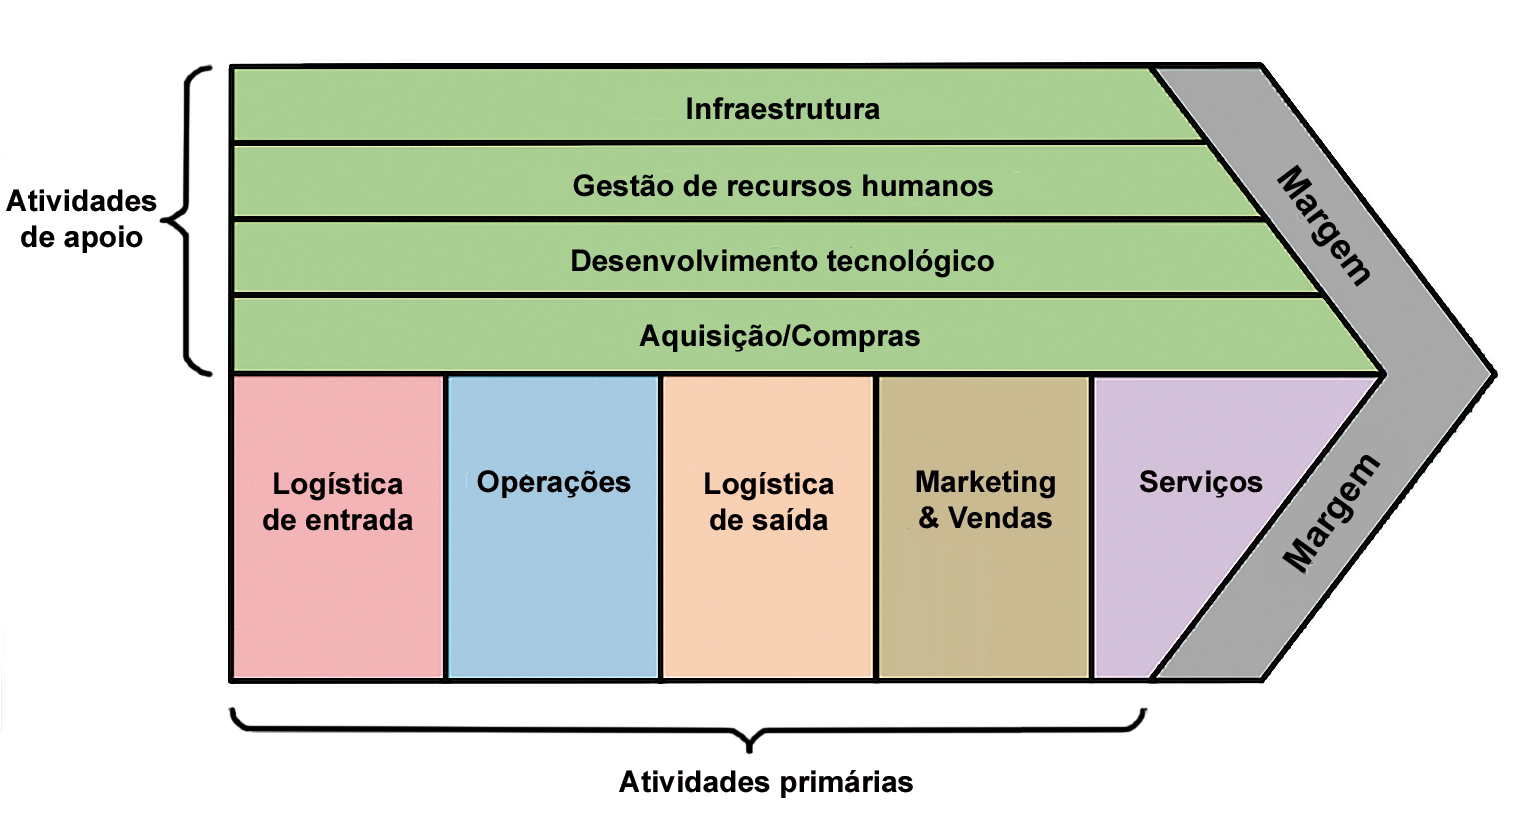
\includegraphics[width=1\textwidth]{porter-cadeia-de-valor.png}
		\label{fig:porter-cadeia-de-valor}
		\source{\citeonline{porter1985competitiveadvantage} (adaptado).}
	\end{figure}
	
	
	As CVs estão focadas em fornecer o máximo valor ao cliente (valor perceptível) com o menor custo e, portanto, é um indicador para a competitividade da empresa. Com o crescente acirramento da competição entre as empresas, essas devem procurar novas formas de agregar mais valor perceptível aos seus produtos, sendo isto em forma de redução de preço, aumento de qualidade, suporte ou qualquer outra nova funcionalidade.
	
	Outra forma de agregação de valor está no princípio de valor compartilhado, que envolve a geração de valor econômico de forma a criar também valor para a sociedade como um todo \cite{porter2011valorcompartilhado} com o enfrentamento de suas necessidades e desafios. Esta necessidade de valor compartilhado parte da percepção generalizada de que empresas prosperam às custas da depreciação da comunidade que as cercam. Soluções que visem o aumento das condições de trabalho, a maior racionalidade e eficiência no tratamento dos recursos naturais necessários para sua atividade e outras formas de balancear o \textit{trade-off} entre eficiência econômica e progresso social são estratégias para se recuperar a legitimidade e a percepção de valor pela sociedade da atividade empresarial.
	
	Atrelado à cadeia de suprimentos e à cadeia de valor existe o conceito de ciclo de vida do produto, que foi um conceito elaborado em meados da década de 1960 com o propósito de criar um modelo que fosse capaz de explicar o sucesso ou fracasso de um produto introduzido ao mercado, sendo capaz também de identificar momentos certos para modificar estratégias de preço, fabricação e quando o produto deve ser descontinuado \cite{cao2012lifecycle}. O modelo inicialmente desenvolvido por \citeonline{levitt1965lifecycle} mostra o padrão de produtos na história passando por quatro estágios bem definidos: desenvolvimento de mercado, crescimento, maturidade e declínio, conforme observado na Figura \ref{fig:product-life-cycle}.
	
	\begin{figure}[H]
		\centering
		\caption{Estágios do ciclo de vida do produto.}
		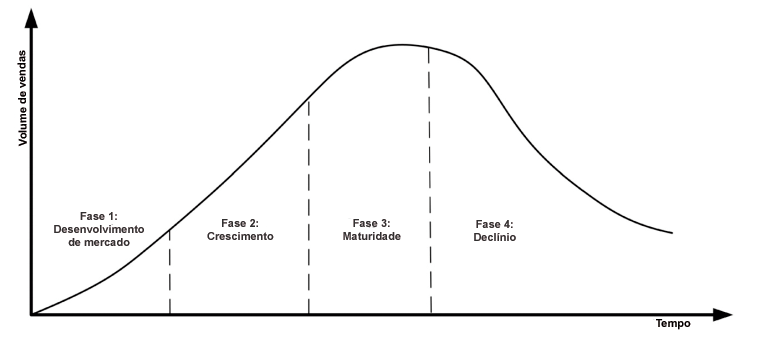
\includegraphics[width=1\textwidth]{product-life-cycle.png}
		\label{fig:product-life-cycle}
		\source{\citeonline{levitt1965lifecycle} (adaptado).}
	\end{figure}

	Vista a tendência global de redução do ciclo de vida do produto devida a rápida taxa de introdução de novas tecnologias para satisfazer a demanda dos clientes, especialmente no mercado de produtos eletrônicos \cite{trappey2008lifecycle}, novas versões de modelos de ciclo de vida do produto vêm sendo elaboradas considerando outros aspectos de mercado e não somente sob a visão da área de \textit{Marketing}. Por vezes, estudos recentes envolvendo ciclo de vida são denominados ``engenharia do ciclo de vida do produto'' (E-CVP) \cite{cao2012lifecycle} e levam em consideração fatores não abordados nos modelos originais como, por exemplo, a fase de pesquisa e desenvolvimento, a retroalimentação de dados, assim como o descarte e reciclagem do produto. Sempre tendo como objetivo auxiliar na tomada de decisões para o sucesso de um produto no mercado.
	
	A Figura \ref{fig:life-cycle-extension} mostra um modelo de ciclo de vida do produto com elementos que incluem a fase de desenvolvimento e a renovação do produto. A renovação do produto e a decorrente extensão de sua vida é essencial, pois mantém o produto no mercado na forma de novas versões e, assim, amplia as receitas mediante ações estratégicas para agregação de valor. O modelo do ciclo de vida e os elementos presentes sempre irão variar conforme a natureza do produto e tipo de mercado consumidor onde o mesmo está inserido.
	
	\begin{figure}[H]
		\centering
		\caption{Modelo de ciclo de vida do produto com renovação do produto.}
		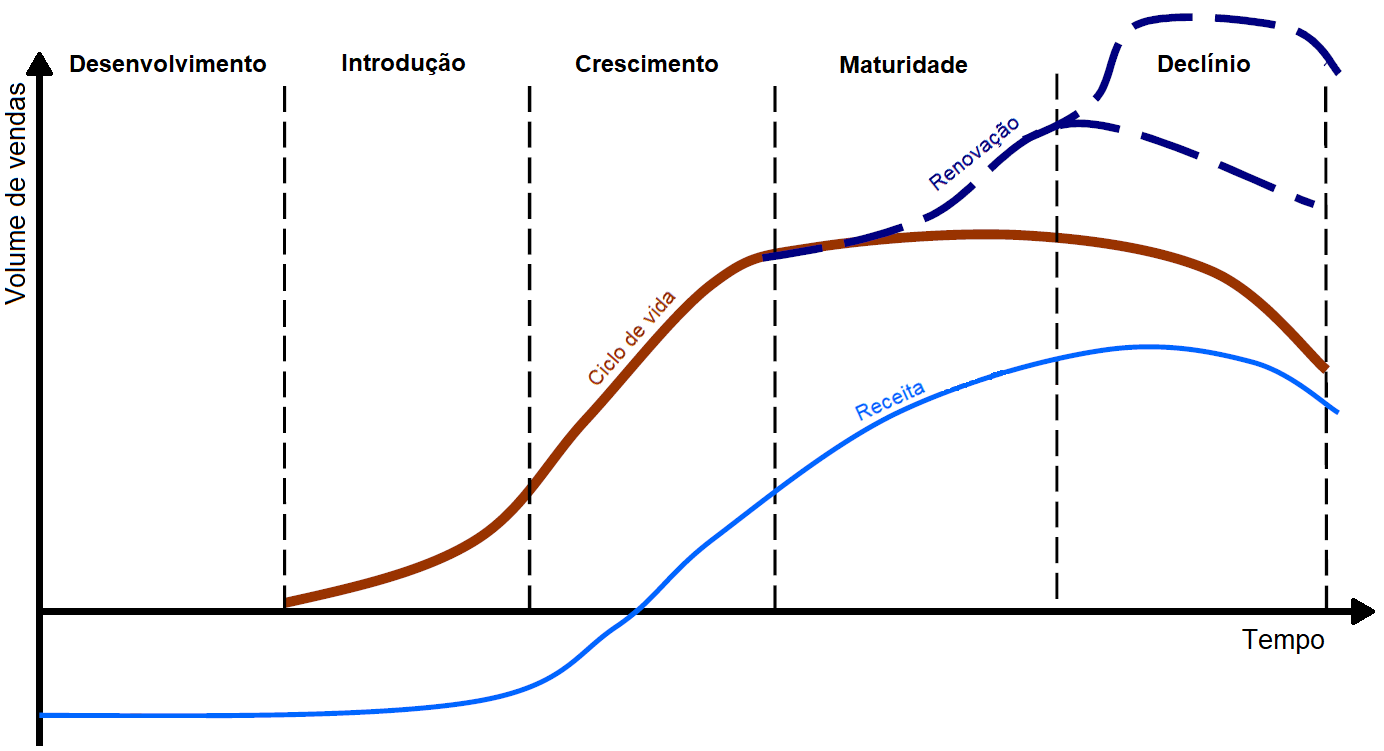
\includegraphics[width=1\textwidth]{life-cycle-extension.png}
		\label{fig:life-cycle-extension}
		\source{\citeonline{liu2010marketingrisk} (adaptado).}
	\end{figure}
	
	Novas propostas de modificações de processos industriais aparecem como formas de se agregar mais valor ao produto/serviço considerando os ciclos de vida do produto cada vez mais curtos. Duas linhas de pesquisas criadas recentemente buscam trazer soluções para os problemas contemporâneos da indústria, como os listados anteriormente, que são os conceitos de Indústria 4.0 (I4.0) e Memória Digital do Produto (MDP).
	
	I4.0 e a MDP são conceitos altamente correlacionados, porém ainda não amplamente abordados em conjunto na literatura, criando assim uma oportunidade de pesquisa a partir de uma lacuna existente.
	
	
\section{Indústria 4.0}

	A crescente integração das Tecnologias da Informação e Comunicação (TIC) às cadeias de valor industriais criou as bases para a próxima revolução industrial chamada Indústria 4.0 \cite{hermann2016design}. Essa mudança de paradigma na indústria se refere às recentes modificações em relação às tecnologias de manufatura, que passam a proporcionar um alto nível de automação e intercâmbio de informações entre equipamentos, produtos e demais atores em um ambiente de manufatura \cite{lasi2014industryfour}. 
	
	O nome Indústria 4.0 (I4.0) se dá ao fato de ser considerada a quarta maior revolução com relação à tecnologia de produção industrial, sendo as ``revoluções industriais'' consideradas evoluções tecnológicas que levaram a grandes mudanças no paradigma de produção, tal histórico de revoluções no campo da indústria é ilustrado na Figura \ref{fig:i4}.

	\begin{figure}[H]
		\centering
		\caption{As revoluções industriais.}
		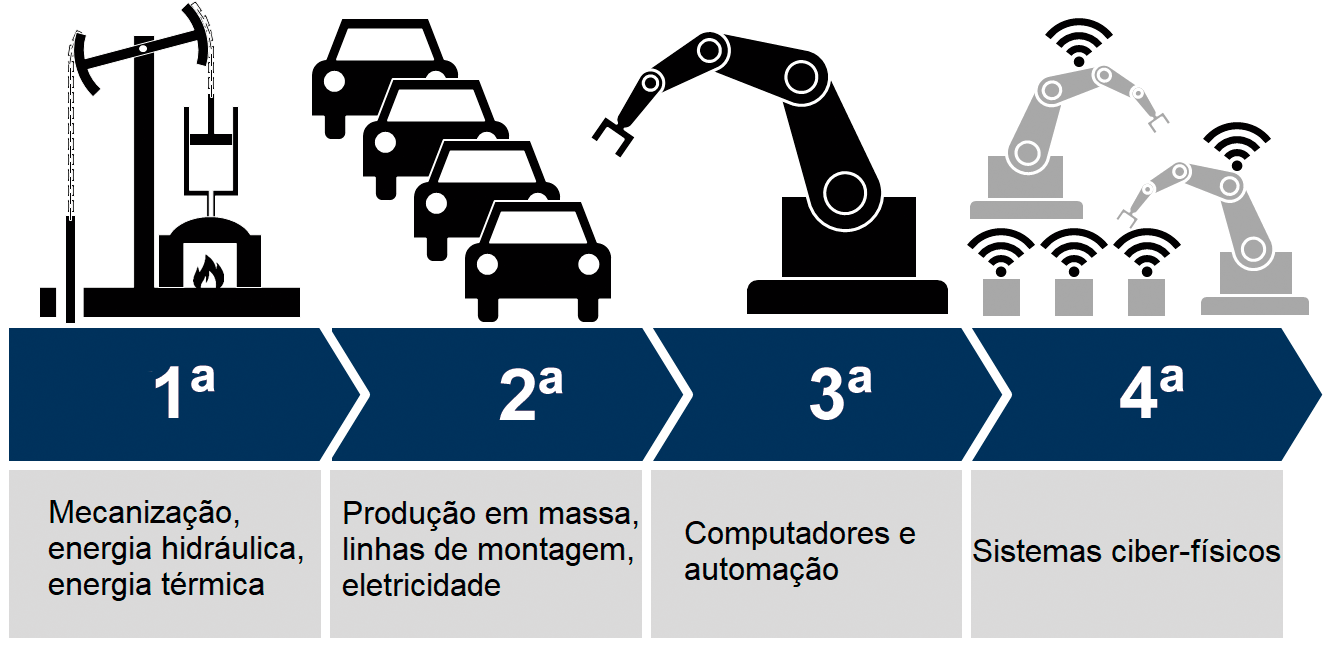
\includegraphics[width=1\textwidth]{i4.png}
		\label{fig:i4}
		\source{\citeonline{lasi2014industryfour} (adaptado).}
	\end{figure}

	Tais modificações na indústria são essenciais devido às novas necessidades da própria indústria e de mudança de padrões de consumo do mercado. Isto acarreta mudanças no cenário operacional destas indústrias. Algumas das causas dessas mudanças operacionais são \cite{lasi2014industryfour}:
	
	\begin{itemize}

		\item Períodos de desenvolvimento curtos: Os períodos de desenvolvimento e inovação de produtos estão sendo reduzidos. A alta capacidade de inovação está se tornando um fator de sucesso para muitas empresas (\textit{Time to market});
		
		\item Individualização sob demanda: Os compradores passam a definir as condições de compra. Essa tendência leva a uma crescente individualização de produtos com características altamente personalizadas e, em casos extremos, a produtos individuais;
		
		\item Flexibilidade: Devido à individualização sob demanda, novas estruturas e organizações na indústria são essenciais para a fabricação de produtos com alto grau de personalização. É necessária uma maior flexibilidade no desenvolvimento do produto, especialmente na produção;
		
		\item Descentralização: Para lidar com condições específicas de cada produto, são necessários procedimentos mais rápidos de tomada de decisão. Para isso, as hierarquias organizacionais precisam ser reduzidas, dando ao produto maior independência sobre seu próprio processo de fabricação;
		
		\item Eficiência de recursos: A maior eficiência sobre o uso dos recursos sempre é algo desejável, porém sua importância se intensifica com as tendências de aumento dos preços dos recursos, bem como a mudança social no contexto de aspectos ecológicos. Isto exige um foco mais intensivo em sustentabilidade, o que decorre em uma maior racionalidade (ou eficiência) na utilização dos recursos.

	\end{itemize}

	Embora o termo I4.0 seja bastante comum na discussão tecnológica atual, muitas empresas, centros de pesquisa e universidades não mantém uma definição comum sobre o assunto. Segundo \citeonline{hermann2016design} e com base em uma revisão de literatura feita pelo mesmo autor, a I4.0 é identificada por quatro princípios de projeto para sua implementação, conforme listados na Tabela \ref{tab:principios-i4}.
	
	
	\begin{table}[H]
		\centering
		\caption{Princípios para implantação da I4.0 baseados em \citeonline{hermann2016design}.}
		\begin{tabular}{|p{1.3in}|p{4in}|}
			
			\hline
			\textbf{Princípio}
			&\textbf{Descrição} \\
			
			\hline
			Interoperabilidade
			& Capacidade das coisas (máquinas, dispositivos, sensores, pessoas, etc) de comunicarem entre si dentro de um sistema por meio de padrões definidos. \\
			
			\hline
			Transparência de informação
			& Tornar acessíveis informações úteis para os demais dispositivos conectados à rede. Informações do mundo virtual como documentos eletrônicos, desenhos, modelos de simulação; e informações sobre o mundo real, como posição, dados de sensores de temperatura, vibração, etc. \\
			
			\hline
			Descentralização de decisões
			& Tomada de decisões baseadas nas informações coletados pelo próprio dispositivo da ao dispositivo autonomia para decidir qual será sua próxima função/operação. Desta forma, um planejamento ou controle central de processos produtivos não se faz essencial e o sistema de produção se torna menos hierarquizado. \\
			
			\hline
			Assistência técnica
			& Devido à complexidade da produção, com redes complexas e tomada decisões descentralizadas, os seres humanos precisam ser auxiliados por sistemas de assistência, de forma a dar compreensibilidade ao processo e às tomadas de decisão necessárias. Os sistemas de assistência devem agregar e tornar visualizável as informações de maneira compreensível.  \\
			\hline
			
		\end{tabular}
		\label{tab:principios-i4}
		\source{O autor.}
	\end{table}

	Os princípios elencados na Tabela \ref{tab:principios-i4} são diretrizes para o desenvolvimento de arquiteturas para a I4.0. As arquiteturas surgem com a necessidade de se definir padrões para a implantação de um sistema. Por ser um assunto novo, as arquiteturas de sistemas produtivos voltadas para a quarta revolução industrial também se encontram em estágio inicial \cite{pisching2018arquitetura}. Hoje, o mais consolidado modelo de arquitetura para a Indústria 4.0 é o RAMI4.0 (Modelo de Arquitetura de Referência para a Indústria 4.0). Esse modelo de arquitetura foi apresentado na feira industrial de Hanôver na Alemanha em abril de 2015.
	
	O RAMI4.0 requer uma representação tridimensional, conforme a Figura \ref{fig:rami4}. Nos três eixos do RAMI4.0 são descritos os níveis hierárquicos de uma fábrica ligada em rede através da Internet (Eixo Níveis Hierárquicos), a representação de arquitetura dos componentes I4.0 (Eixo Camadas) e o ciclo de vida de instalações e de produtos (Eixo Ciclo de Vida e Cadeia de Valor).
	
	\begin{figure}[H]
		\centering
		\caption{Representação do RAMI4.0.}
		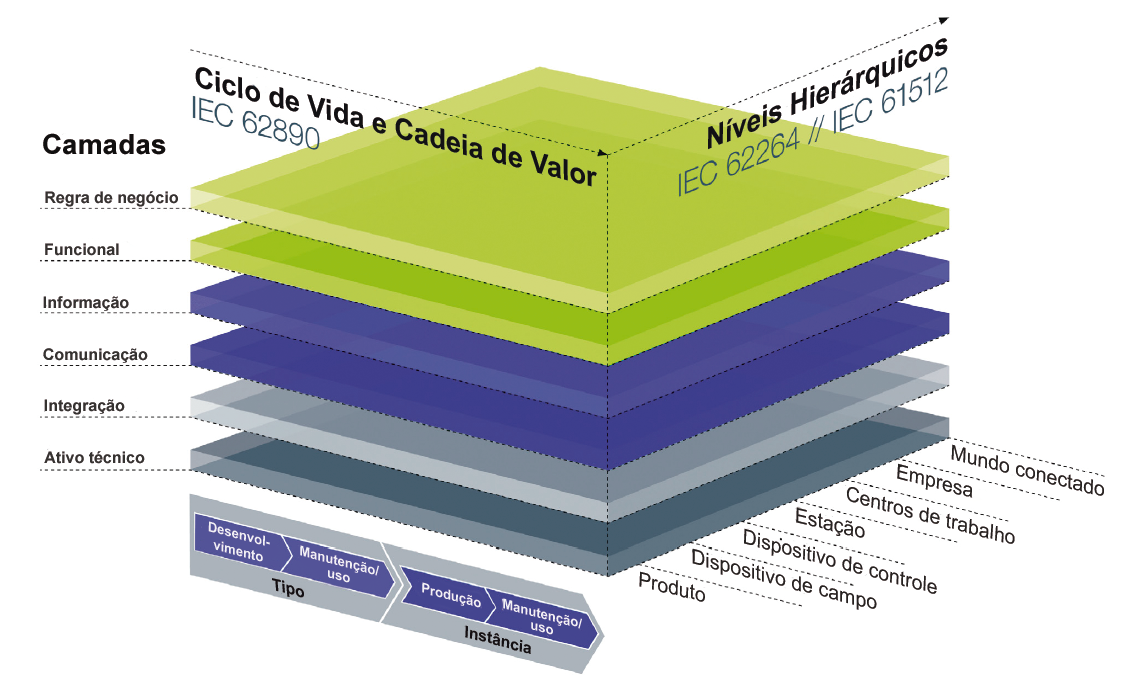
\includegraphics[width=1\textwidth]{rami4.png}
		\label{fig:rami4}
		\source{\citeonline{adolphs2015rami} (adaptado).}
	\end{figure}

	O RAMI4.0, como um modelo de referência, é um elemento para padronização do projeto e implantação de aplicações em I4.0. O RAMI4.0 é uma padronização de linguagem e deve ser aceito e usados por todos os participantes para protótipo, desenvolvimento e validação.

\section{Memória Digital do Produto}

	O termo ``Memória Digital do Produto'' (MDP) surgiu pela primeira vez em 2007 por meio de um boletim de notícias de tecnologia de uma empresa alemã fabricante de conectores elétricos e eletrônicos \cite{wahlster2007digitalmemory}. À época, o termo foi tratado com analogia a um diário, que mantinha todas as informações do produto ao longo de seu ciclo de vida.

	Hoje, o conceito na literatura se refere a sistemas que permitem a coleta de dados em todas as fases do ciclo de vida do produto para a distribuição e/ou análise. Os dados de interesse do produto podem ser relativos a qualquer fase do produto ao longo de sua cadeia de valor, o que abrange dados de produção individual, de montagem, de distribuição, de uso por parte do consumidor, etc. A Figura \ref{fig:MDP-ideia} ilustra o conceito de MDP.
	 
	\begin{figure}[H]
		\centering
		\caption{Coleta de dados do produto ao longo da cadeia de valores.}
		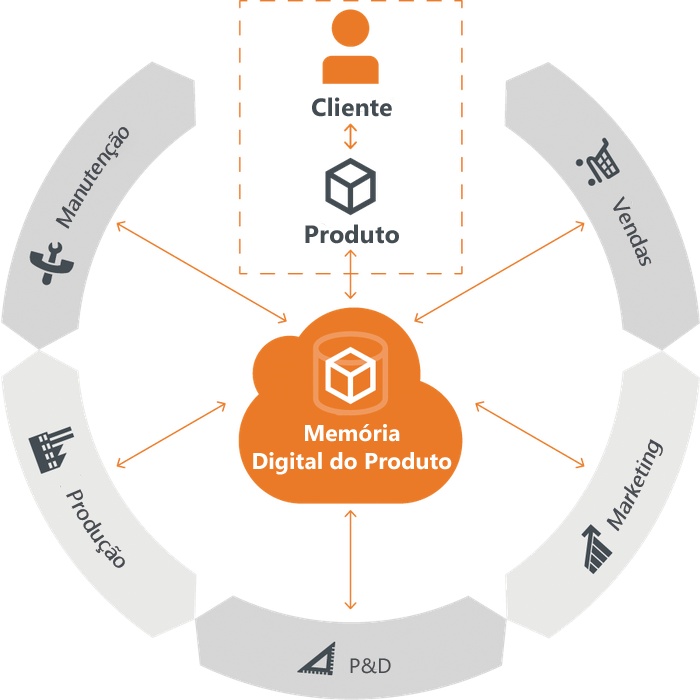
\includegraphics[width=0.6\textwidth]{MDP-ideia.png}
		\label{fig:MDP-ideia}
		\source{\citeonline{zuhlke2020digitalmemory} (adaptado).}
	\end{figure}

	Sua relevância está no fato da tendência de produtos novos apresentarem ciclos de vida cada vez mais curtos e devido ao fato das cadeias de suprimentos apresentarem redes cada vez mais complexas, com múltiplos fornecedores e clientes. Com isso, a MDP manteria registros digitais do ciclo de vida dos produtos, faria o monitoramento constante do seu estado atual e realizaria o rastreamento de sua posição. Segundo \citeonline{wahlster2007digitalmemory}, o acesso a essas informações pelas partes interessadas seria de vital importância na competitividade de empresa produtoras e de comércio, além de abrir novas proteções em relação à pirataria.
	
	A implementação de uma memória com informações sobre produto ao longo de sua cadeia de valores é importante, pois torna possível acessar e utilizar informações do mundo real providenciada por diferentes fontes ao longo da cadeia de suprimentos para o potencial benefício das partes interessadas naquele produto \cite{brandherm2011productmemory}, como, por exemplo, fabricantes, transportadores, varejistas e consumidores. 
	
\section{Interrelação entre I4.0 e MDP}

 	Ambos os conceitos de I4.0 e MDP são conceitos recentes, surgidos em 2011 \cite{kagermann2011industrie} e 2007 \cite{wahlster2007digitalmemory}, respectivamente . A área multidisciplinar de estudo envolvendo MDP e I4.0 surgira em 2013 com o projeto SemProM \cite{wahlster2013semprom}, porém ainda quando I4.0 era um conceito abrangente e sem diretrizes concretas para sua implementação, que ocorreria em 2013 por meio do documento de recomendações para implementação da iniciativa estratégia Industrie 4.0 \cite{kagermann2013recommendations}; e sem a criação do modelo de arquitetura de referência para Indústria 4.0 (RAMI4.0), que seria divulgada em 2015 por meio do documento entitulado ``RAMI4.0'', divulgado por um periódico alemão \cite{hankel2015rami}.
 	
 	 Alguns outros estudos como \citeonline{lasi2014industryfour} citam MDP como oportunidade de estudo e aplicação dentro da I4.0, outros como \citeonline{weyer2015standardization} e \citeonline{paelke2014augmented} implementam sistemas práticos envolvendo ambos os conceitos, porém sem considerações sobre cadeia de valor.
 	
	Há estudos na área multidisciplinar de I4.0 e MDP, principalmente no meio acadêmico, empresarial e governamental alemão pelo fato de esses conceitos terem surgido na Alemanha. Porém nenhum trabalho até o presente momento relaciona o modelo de arquitetura de referência para a I4.0 (RAMI4.0) com a MDP, o que aponta uma lacuna de conhecimento dentro de I4.0 a ser explorada.
	
	Estudos sobre o RAMI4.0 são importantes no sentido de padronizar a implementação da I4.0 em empresas de diferentes negócios, garantindo assim a interoperabilidade dos serviços. O eixo ``Ciclo de Vida e Cadeia de Valor'' apresenta diretrizes para o correto planejamento da vida de um produto e sugere cenários para criação de valor perceptível ao produto/serviço. Integrar o conceito de MDP ao RAMI4.0, especificamente ao eixo de ``Ciclo de Vida e Cadeia de Valor'', enriquece o nível de discussão sobre essa arquitetura de referência e dá mais robustez ao modelo para uma futura adoção generalizada por parte de empresas por todo o mundo.
	
	A ``Plattform Industrie 4.0'' é uma das principais redes mundiais de discussão sobre I4.0 \cite{kagermann2013recommendations, acatech2014plattform, germany2019plattform}. O Conselho de Pesquisa da Plattform Industrie 4.0 é o comitê consultivo estratégico da Plattform Industrie 4.0 e identifica necessidades de pesquisa e ações em torno da I4.0. O comitê identificou e definiu quatro temas-chave de abordagens no setor tecnológico, econômico, metodológico e social/legal para se implementar com sucesso a I4.0 \cite{hirsch-kreinsen2019keythemes}, conforme mostrado na Figura \ref{fig:keythemes-i4}. Isso significa que os tópicos elencados são temas com alto potencial para a otimização de rotinas e processos de produção existentes no cenário de I4.0.
	
	\begin{figure}[H]
		\centering
		\caption{Temas-chave de pesquisa e desenvolvimento em I4.0.}
		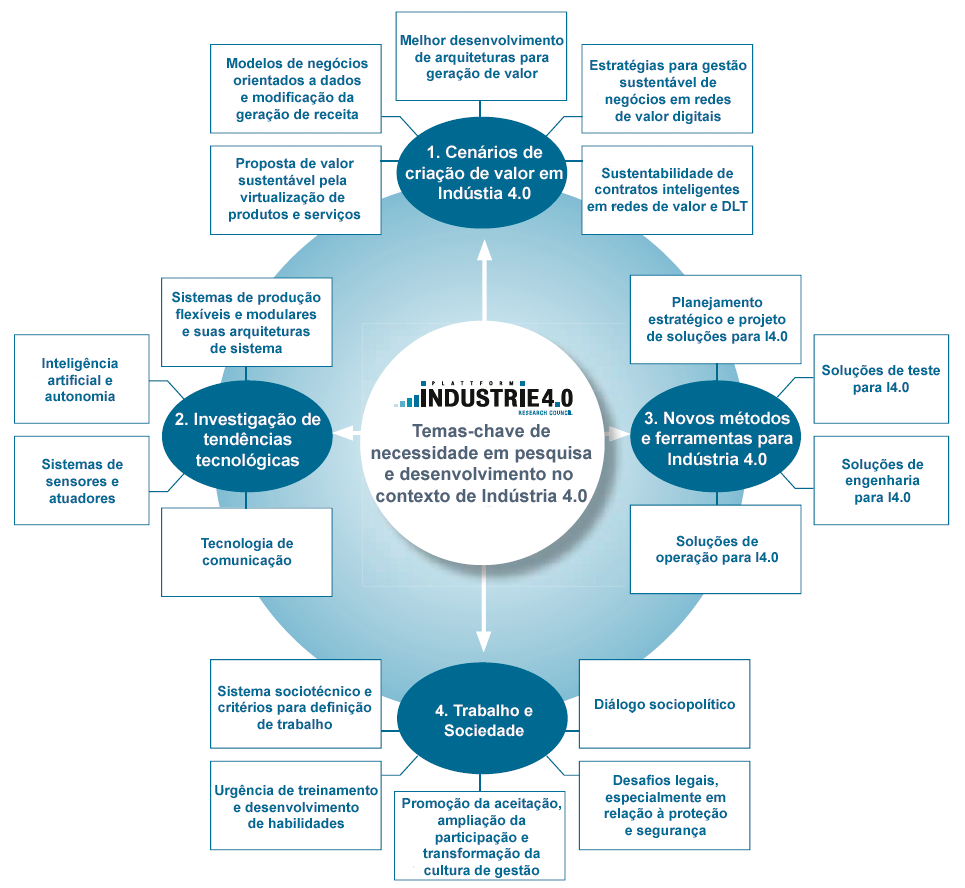
\includegraphics[width=1\textwidth]{keythemes-i4.png}
		\label{fig:keythemes-i4}
		\source{\citeonline{hirsch-kreinsen2019keythemes}.}
	\end{figure}

	Dentre os temas elencados na Figura \ref{fig:keythemes-i4}, destacam-se os subitens relacionados ao tópico ``Cenários de criação de valor em Indústria 4.0'' por estarem altamente relacionados ao RAMI4.0 e ao conceito de geração de valor por meio da MDP. O desenvolvimento de arquiteturas para geração de valor e a criação de negócios orientados a dados são temas de grande oportunidade dentro do cenário de I4.0, especialmente se considerando os métodos quantitativos de \textit{Business Intelligence} e de análise de dados já estabelecidos.
	

\section{Objetivos da pesquisa}

	O objetivo do trabalho de pesquisa é a investigação da integração do conceito de MDP ao RAMI4.0, especificamente ao eixo de ``Ciclo de Vida e Cadeia de Valor'', de forma a se aperfeiçoar a elaboração dessa arquitetura a fim de proporcionar mais robustez ao modelo para uma futura adoção generalizada por parte de empresas por todo o mundo.
	
	Todo o estudo é feito com a proposta de aperfeiçoar o RAMI4.0 no sentido de propiciar o surgimento de novos cenários de criação de valor no contexto de I4.0 e incentivar geração de novos modelos de negócio baseado em dados.
	
	Este plano de pesquisa envolve o estudo de diversos temas relacionados à Indústria 4.0. Os principais itens estão explicitados a seguir. Diversos novos itens são adicionados ao foco de pesquisa à medida que há aprofundamento nos itens abaixo.
	
	\begin{itemize}
		\item Indústria 4.0;
		\item RAMI4.0;
		\item Cadeia de valor;
		\item Ciclo de vida do produto;
		\item Memória digital do produto;
		\item Internet das coisas.
	\end{itemize}
	
	Tais temas são estudados a fim de se analisar o estado da arte atual em I4.0 e a partir disso propor alterações sobre o RAMI4.0 incluindo o conceito de MDP.





























% ----------------------------------------------------------
\chapter{Metodologia}

	O trabalho é executado a partir de revisão bibliográfica de textos acadêmicos, como dissertações e teses, artigos publicados em revistas acadêmicas, livros teóricos e notas de estudos técnicos. A revisão bibliográfica tem o objetivo de se inteirar do estado da arte das tecnologias envolvidas na Indústria 4.0.
	
	As disciplinas obrigatórias do programa de pós-graduação cursadas durante o período do mestrado foram selecionadas com base na relevância e relacionamento com a natureza da pesquisa em Indústria 4.0 e incluem disciplinas também de outros programas de pós-graduação, como o de Engenharia Elétrica, Engenharia de Transportes e Engenharia de Produção.
	
	A metodologia adotada neste projeto será baseada naquela proposta por \citeonline{jensen1997petrinet}, onde as etapas de pesquisa são compostas por um ciclo repetitivo de três aspectos, sendo elas as teorias, ferramentas e aplicações, conforme ilustrado na Figura \ref{fig:metodologia-jensen}.
	
	O próprio conhecimento adquirido nas disciplinas por meio da aprendizagem de novas “ferramentas” pode modificar parte das “aplicações” e com isso realimentar as “teorias” iniciais. Mediante a evolução do projeto ao longo do tempo, novas propostas surgem, e com isso a necessidade do aprendizado de novos conceitos/teorias.

	\begin{figure}[H]
		\centering
		\caption{Metodologia de pesquisa utilizada.}
		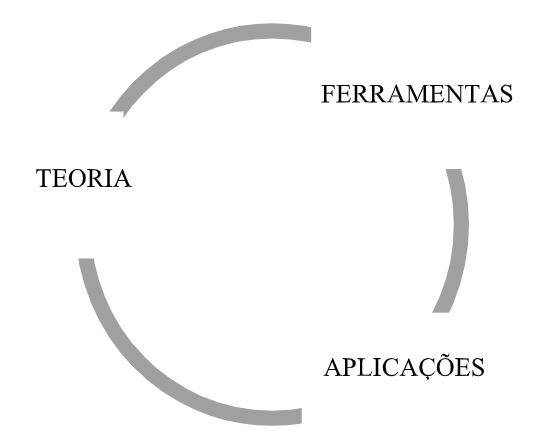
\includegraphics[width=0.7\textwidth]{metodologia-jensen.png}
		\label{fig:metodologia-jensen}
		\source{\citeonline{jensen1997petrinet} (adaptado).}
	\end{figure}

	Aplicando-se a metodologia proposta por \citeonline{jensen1997petrinet} para o caso específico do plano de pesquisa em questão, pode-se listar teorias, ferramentas e aplicações individuais do projeto, formando-se o ciclo mostrado na Figura \ref{fig:metodologia-jensen}. Os três aspectos identificados na Figura \ref{fig:metodologia-jensen} devem evoluir simultaneamente, recondicionando-se mutuamente.






% ----------------------------------------------------------
\chapter{Fundamentos}

	

\section{Gestão do ciclo de vida do produto}

	A gestão do ciclo de ciclo de vida do produto (GCVP) refere-se ao manuseio de um bem ao longo de seu caminho pelos estágios típicos de sua vida útil: desenvolvimento e introdução, crescimento, maturidade / estabilidade e declínio, conforme observado na Figura \ref{fig:product-life-cycle}. No GCVP, o manuseio se refere às etapas de fabricação, comercialização, uso e qualquer outra fase em que o produto se encontra. A GCVP tem como finalidade auxiliar gestores na tomada de decisões de negócios com estratégias como políticas de preços, expansão de mercado, retirada do produto ou inserção de novas versões, etc.
	
	GCVP é o sistema de gerenciamento dos produtos de uma empresa. Sua função não é gerenciar apenas um de seus produtos, mas gerenciar de maneira integrada todas as suas partes assim como o portfólio de produtos da empresa \cite{stark2015lifecycle}.
	
	Em nível mais alto, o objetivo do GCVP é aumentar as receitas do produto, reduzir os custos relacionados ao produto, maximizar o valor do portfólio de produtos e maximizar o valor dos produtos atuais e futuros para clientes e acionistas \cite{stark2015lifecycle}.

\pagebreak
\section{Indústria 4.0}

	Indústria 4.0 (I4.0) é o nome dado às recentes modificações em relação às tecnologias utilizadas em processos processos industriais. Tais tecnologias são inseridas com o propósito de se oferecer um alto nível de automação e intercâmbio de informações entre equipamentos e produtos.

	O nome I4.0 se dá pelo fato de ser considerada a quarta grande revolução com relação às tecnologias de produção industrial, sendo as ``revoluções industriais'' consideradas evoluções tecnológicas que levaram a grandes mudanças no paradigma de produção. As outras transições dentro da indústria ao longo da história aconteceram: no campo da mecanização (1ª revolução industrial), com relação ao intenso uso da energia elétrica (2ª revolução industrial) e com a expansão da digitalização (3ª revolução industrial) \cite{lasi2014industryfour}. Tal histórico de revoluções no campo da indústria é ilustrado na Figura \ref{fig:i4-2}.

	\begin{figure}[H]
		\centering
		\caption{Evolução do grau de complexidade da indústria por meio das revoluções industriais.}
		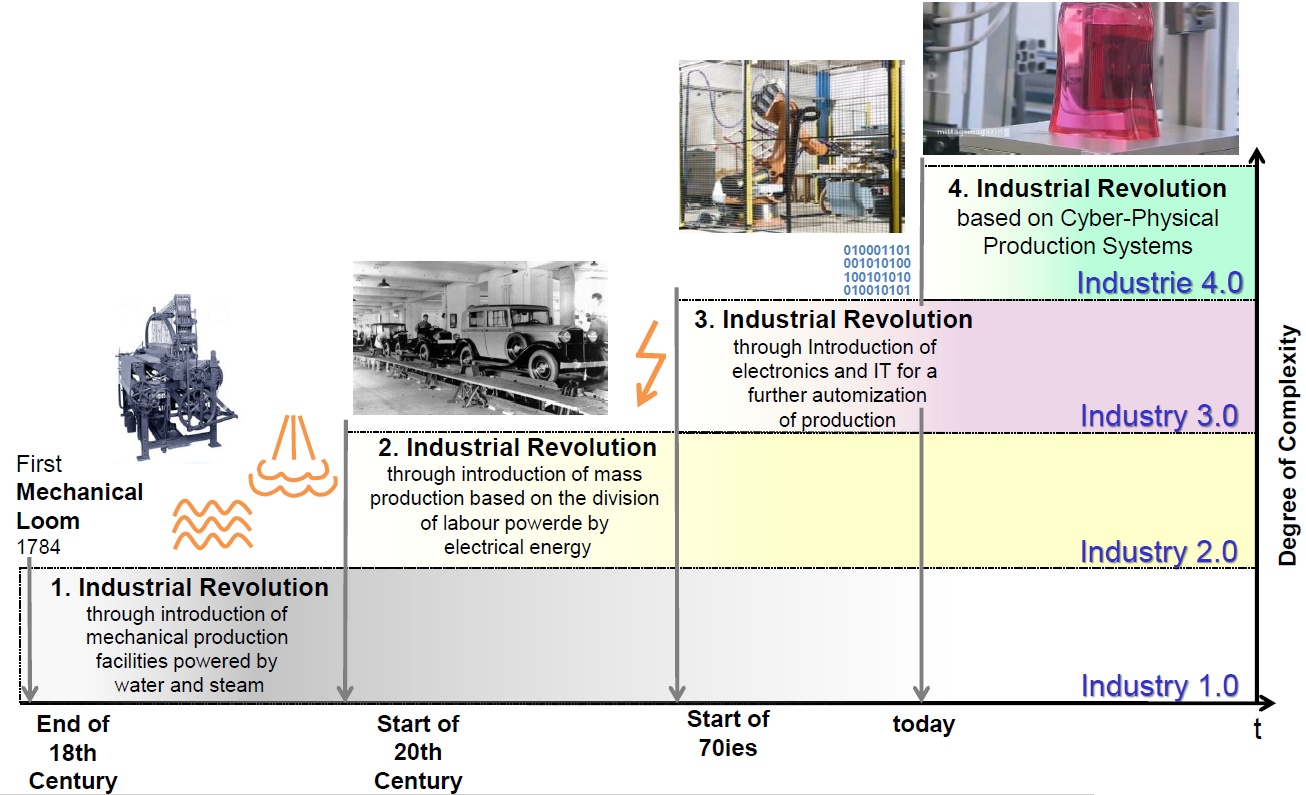
\includegraphics[width=1\textwidth]{i4-2.png}
		\label{fig:i4-2}
		\source{\citeonline{wahlster2013industrie} }
	\end{figure}

	O termo I4.0 foi trazido a público pela primeira vez em 2011 na feira industrial de Hanôver (\textit{Hannover-Messe}) \cite{kagermann2011industrie}, que é uma feira tecnológica de grande relevância internacional e tem o costume de apresentar grandes inovações relacionadas ao setor industrial.

	Por vezes, a I4.0 é tratada também como a convergência da produção industrial com as novas Tecnologias de Informação e Comunicação (TIC) \cite{hermann2016design}.

	A quarta revolução industrial já está em curso segundo Fórum Mundial Econômico \cite{schwab2016fourth} em seu encontro anual realizado em Davos no ano de 2016 e as razões para o surgimento deste novo paradigma de produção incluem: a competição acirrada entre empresas, alta complexidade de manufatura dos produtos e seus altos níveis de personalização do produto por parte dos clientes \cite{bordeleau2018bi, vaidya2018industryfour}.

	Uma das bases para este novo paradigma de produção é a interligação de objetos no ambiente de produção por meio de identificadores individuais por meio dos conceitos de Internet das Coisas (\textit{Internet of Things} - IoT) e de Internet das Coisas Industrial (\textit{Industrial Internet of Things} - IIoT). Tais ``objetos'' se referem a equipamentos, produtos, máquinas, peças, pessoas e quaisquer outros elementos envolvidos no ambiente industrial, por vezes também são denominados ``ativos''.
	
	Esses ativos são inseridos no meio digital, onde podem trocar informações entre si e executarem comandos de funções sob seu respectivo correspondente físico de forma mais autônoma e com menor intervenção humana por meio do uso extensivo de recursos avançados de tecnologias da informação e comunicação \cite{adolph2018roadmap}. Devido a essa maior relação entre elementos do sistema de fabricação, extingui-se a relação essencialmente hierarquizada da indústria tradicional e os ativos passam a deter a capacidade de se comunicarem diretamente com outros elementos de diferentes níveis, conforme ilustrado na Figura \ref{fig:i3-to-i4}.
	
	\begin{figure}[H]
		\centering
		\caption{Transição do modelo hierárquico tradicional (a)) para o modelo flexível de comunicação entre dispositivos na Indústria 4.0 (b).}
		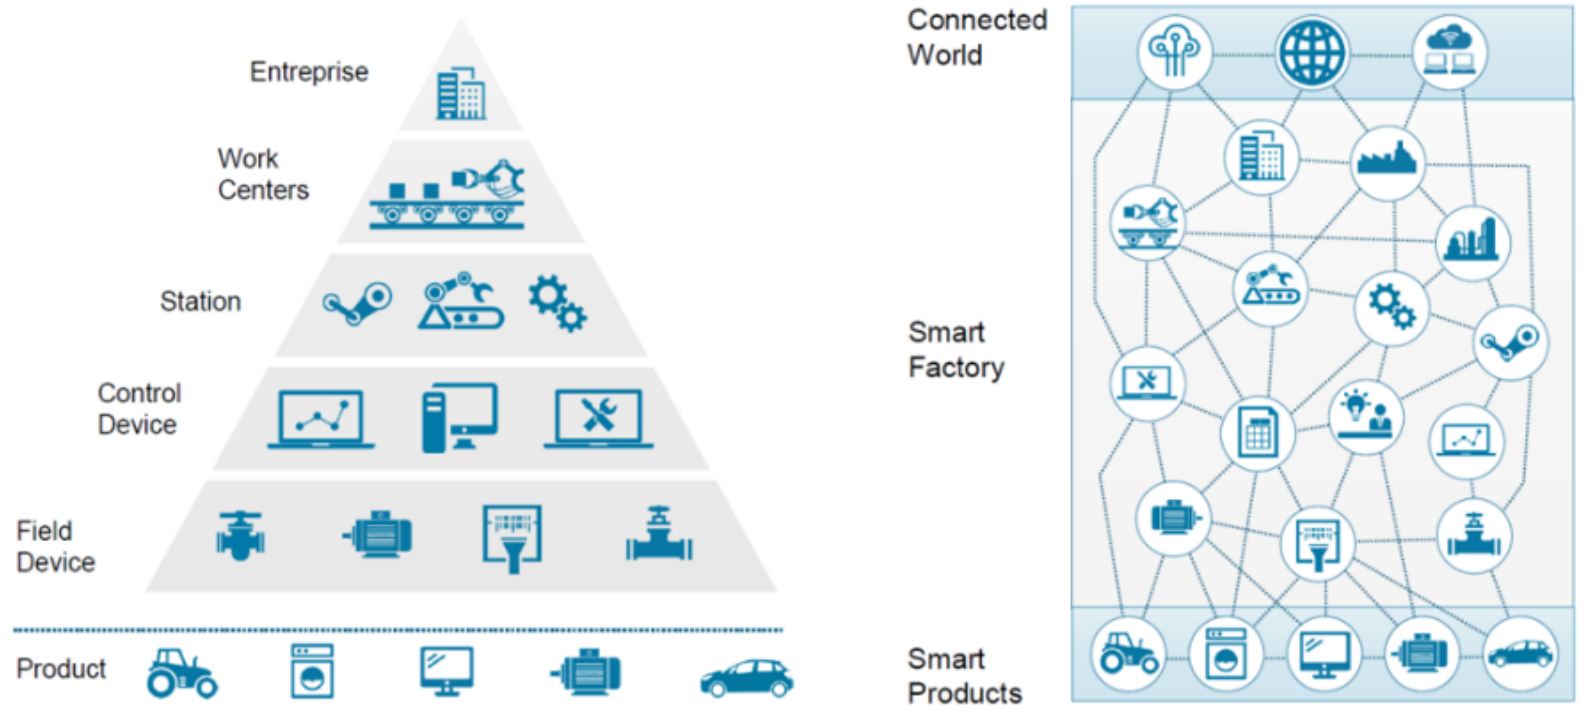
\includegraphics[width=1\textwidth]{i3-to-i4.png}
		\label{fig:i3-to-i4}
		\source{\citeonline{schmittner2017mtom} (adaptado).}
	\end{figure}

	Essa automatização e a troca de informações entre os ativos tem grande potencial de dar mais eficiência aos processos industriais, pois desta forma o sistema pode tomar decisões ótimas com base nas informações que lhe foram fornecidas por meio de sensores e identificadores. A visão para o futuro da produção baseado na I4.0 envolve sistemas de manufatura modulares e eficientes em cenários nos quais os produtos controlam seus próprios processos de fabricação \cite{lasi2014industryfour}.
	
	Há uma tendência global de redução do ciclo de vida do produto devida à rápida introdução de novas tecnologias para satisfazer a demanda dos clientes, especialmente em produtos eletrônicos \cite{trappey2008lifecycle}. A I4.0 beneficia a chegada de produtos com curto ciclo de vida uma vez que o produto controla seu próprio processo de fabricação, beneficiando assim ajustes e personalização por parte do cliente, enquanto preserva os custos, a qualidade e o tempo de aprovisionamento (\textit{lead time}) da produção em massa.
	
	Indústria 4.0 é um conceito. Isto significa que são princípios a serem seguidos e implementados, porém o caminho para a implementação, assim como as tecnologias a serem adotadas podem ser diversas. As peculiaridades de cada indústria e de cada mercado estabelecem diferentes regras de negócios e, portanto, cada setor da indústria pode necessitar de diferentes formas e tecnologias para se implementar a I4.0 e se tornar uma fábrica inteligente. Alguns avanços tecnológicos, entretanto, são muito importantes ou essenciais para a implementação da I4.0 em qualquer sistema de manufatura, alguns deles são mostrados na Figura \ref{fig:tecnologias-i4}.
	
	\begin{figure}[H]
		\centering
		\caption{Avanços tecnológicos que moldam a I4.0.}
		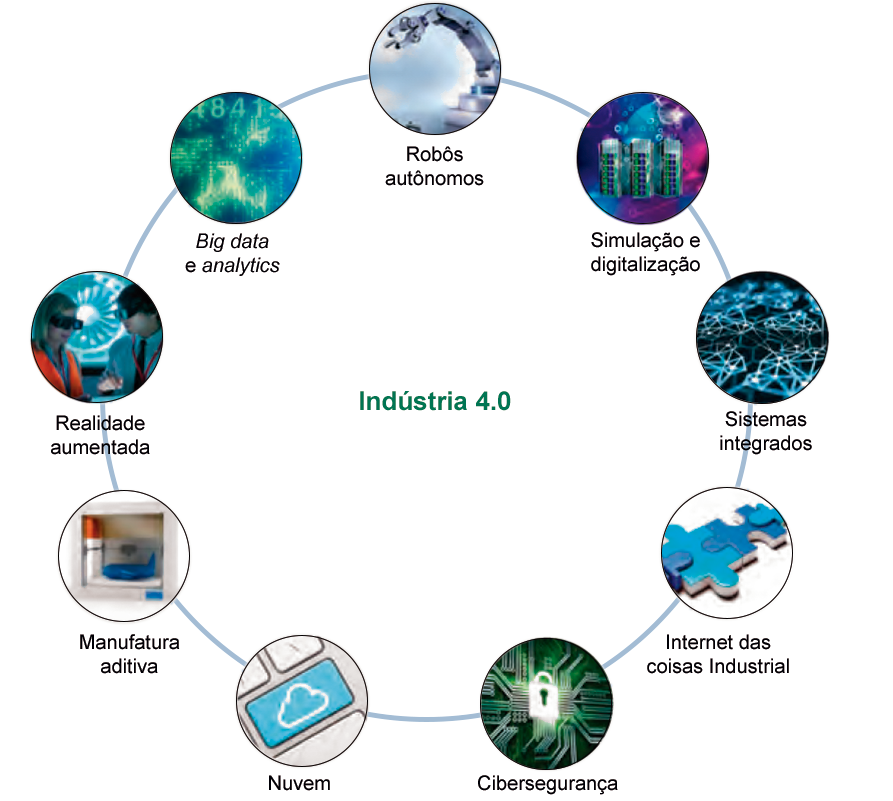
\includegraphics[width=1\textwidth]{tecnologias-i4.png}
		\label{fig:tecnologias-i4}
		\source{\citeonline{russmann2015industryfour} (adaptado).}
	\end{figure}

	Após a primeira aparição do termo I4.0 na feira industrial de Hanôver em 2011, o termo ganhou significativa popularidade, principalmente no meio acadêmico e empresarial alemão. O termo foi então incentivado pelo governo alemão \cite{lasi2014industryfour, kagermann2013recommendations}, que apoiou a ideia e anunciou a Indústria 4.0 como parte integral de sua iniciativa estratégica para a indústria alemã, visando liderança em inovação tecnológica \cite{drath2014industrie} como uma abordagem para fortalecer a competitividade da indústria manufatureira alemã.	

	Por meio da iniciativa \textit{Plattform Industrie 4.0}, criada em 2013 pelo Ministério Federal da Educação e Pesquisa (\textit{Bundesministerium für Bildung und Forschung}) \cite{germany2019plattform} e com o grupo de trabalho ``Industrie 4.0 Working Group'' em comunicação com diversas associações de engenharia e indústrias alemãs, foram criados documentos oficiais como o ``\textit{Recommendations for implementing the strategic initiative Industrie 4.0}'' \cite{kagermann2013recommendations}, o ``\textit{German Standardization Roadmap - Industrie 4.0}'' \cite{adolph2018roadmap} e o ``\textit{Implementation Strategy Industrie 4.0}'' \cite{bitkom2016implementation} publicados em inglês com normas e diretrizes para a implementação da I4.0. Esta iniciativa atrelada ao entusiasmo acadêmico em torno do projeto I4.0 disseminaram o conceito fora da área de língua alemã e popularizou o termo I4.0 no mundo todo como epônimo de um futuro projeto no contexto de indústrias de alta tecnologia.

	O impacto econômico dessa revolução industrial deve ser enorme, pois a I4.0 promete uma eficiência operacional substancialmente maior, bem como o desenvolvimento de modelos, serviços e produtos de negócios totalmente novos \cite{hermann2016design}.
	
	Em revoluções industriais passadas, os países pioneiros a se adaptarem às drásticas mudanças de produção foram os que mais se beneficiaram e se consolidaram como potências econômicas. Na quarta revolução industrial não será diferente. Embora a mudança completa para a I4.0 possa levar 20 anos para ser concretizada \cite{russmann2015industryfour}, nos próximos anos serão estabelecidos avanços importantes que definirão os pioneiros e detentores de tecnologias dessa nova revolução. Portanto, é de interesse de cada país liderar a concorrência global por meio de sua consolidação como mercado líder e fornecedor de soluções para a Indústria 4.0.

	\pagebreak
	\subsection{Modelo de Arquitetura de Referência para a Indústria 4.0}
	
	O Modelo de Arquitetura de Referência para a Indústria 4.0, abreviado RAMI4.0, consiste em um sistema de coordenadas tridimensional que descreve todos os aspectos cruciais da Indústria 4.0. Dessa maneira, inter-relações complexas podem ser divididas em grupos menores e mais simples.
	
	A Figura \ref{fig:rami4} mostra a representação do RAMI4.0 e especifica os itens contidos em cada eixo. A Tabela \ref{tab:rami-eixos} detalha a função de cada eixo do RAMI4.0.
	
	\begin{table}[H]
		\centering
		\caption{Eixos do RAMI4.0}
		\begin{tabular}{|p{1.3in}|p{4in}|}
			
			\hline
			\textbf{Eixo}
			&\textbf{Descrição} \\
			
			\hline
			Camadas
			& As seis camadas no eixo vertical servem para descrever a decomposição de um ativo em suas propriedades, isto é, o mapeamento virtual de um ativo. Tais representações se originam da tecnologia da informação e comunicação, onde as propriedades de sistemas complexos são comumente divididas em camadas. \\
			
			
			\hline
			Ciclo de vida e  Cadeia de valor
			& O eixo horizontal esquerdo representa o ciclo de vida das instalações e produtos, com base na IEC 62890 para gerenciamento do ciclo de vida. Além disso, é feita uma distinção entre ``tipos'' e ``instâncias''. Um ``tipo'' se torna uma ``instância'' quando o projeto e a prototipagem são concluídos e o produto real está sendo fabricado. \\
			
			\hline
			Níveis hierárquicos
			& No eixo horizontal direito estão indicados os níveis hierárquicos da IEC 62264, a série de padrões internacionais para sistemas de TI e controle corporativos. Esses níveis hierárquicos representam as diferentes funcionalidades das fábricas ou instalações. Para representar o ambiente I4.0, essas funcionalidades foram expandidas para incluir o produto da manufatura, rotuladas como ``Produto'', e a conexão com a IoT, denominada ``Mundo conectado''. \\
			\hline
			
		\end{tabular}
		\label{tab:rami-eixos}
		\source{O autor.}
	\end{table}

	A Figura \ref{fig:eixo_layers} mostra o eixo Camadas do RAMI4.0.
	
	\begin{figure}[H]
		\centering
		\caption{Eixo Camadas do RAMI4.0.}
		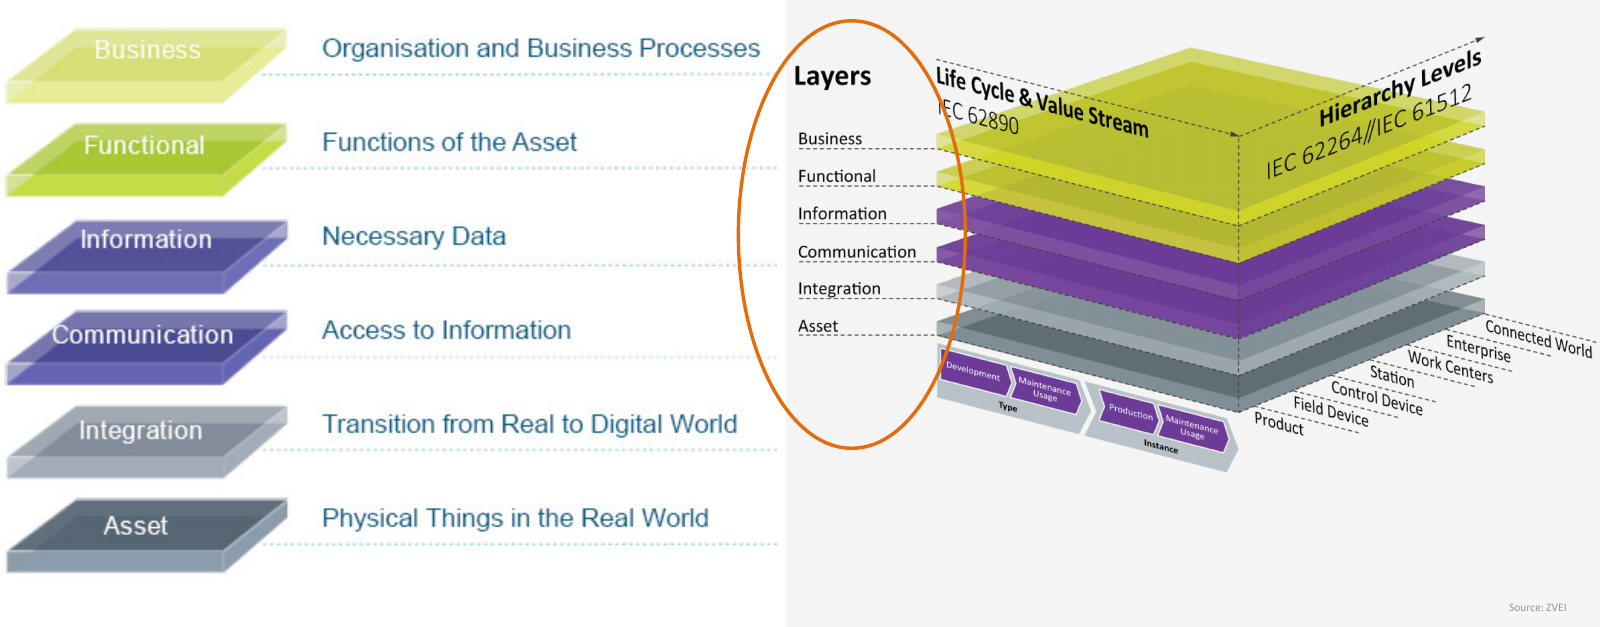
\includegraphics[width=1\textwidth]{eixo_camadas.png}
		\label{fig:eixo_camadas}
		\source{\citeonline{germany2018ramistandardization} (adaptado).}
	\end{figure}

	A Figura \ref{fig:eixo_niveishierarquicos} mostra o eixo Níveis Hierárquicos do RAMI4.0.
	
	\begin{figure}[H]
		\centering
		\caption{Eixo Níveis Hierárquicos do RAMI4.0.}
		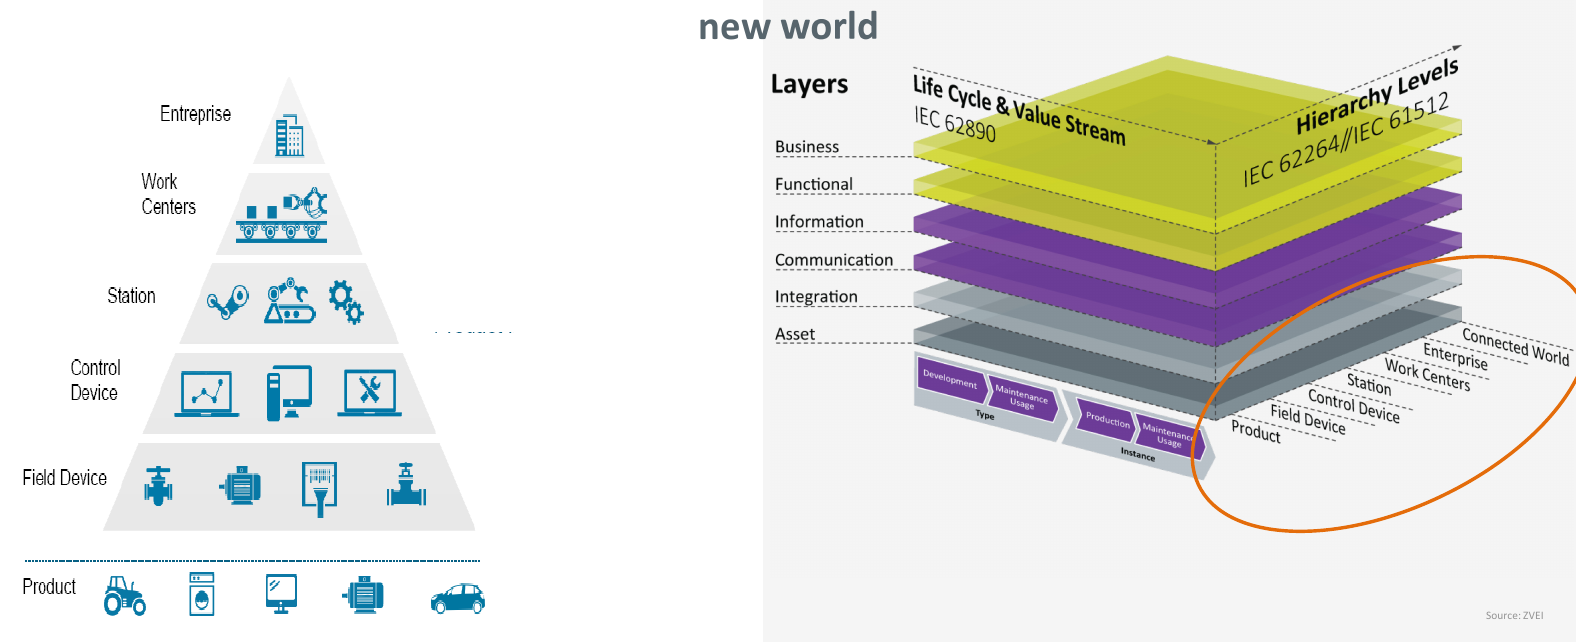
\includegraphics[width=1\textwidth]{eixo_niveishierarquicos.png}
		\label{fig:eixo_niveishierarquicos}
		\source{\citeonline{germany2018ramistandardization} (adaptado).}
	\end{figure}

	A Figura \ref{fig:eixo_ciclodevida} mostra o eixo Ciclo de Vida e Cadeia de Valor do RAMI4.0.
	
	\begin{figure}[H]
		\centering
		\caption{Eixo Ciclo de Vida e Cadeia de Valor do RAMI4.0.}
		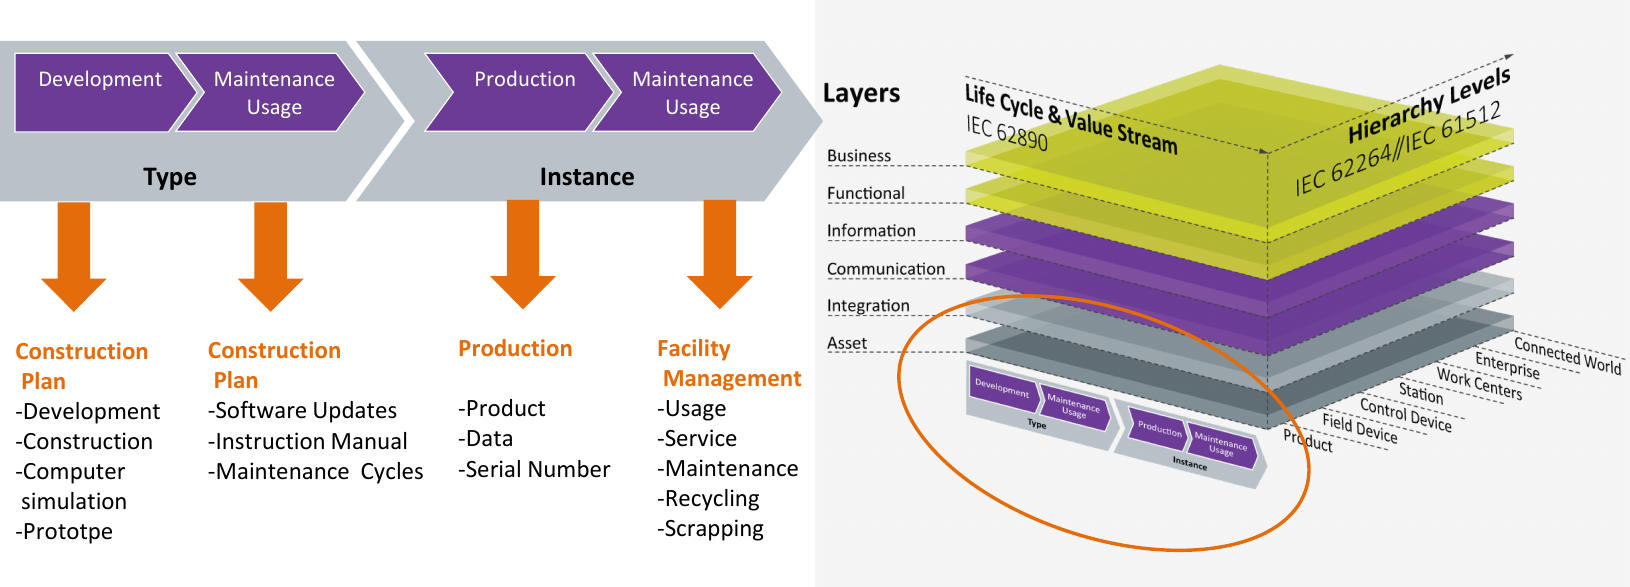
\includegraphics[width=1\textwidth]{eixo_ciclodevida.png}
		\label{fig:eixo_ciclodevida}
		\source{\citeonline{germany2018ramistandardization} (adaptado).}
	\end{figure}

	
	
	Dentro desses três eixos, todos os aspectos cruciais da I4.0 podem ser mapeados, permitindo que objetos como máquinas sejam classificados de acordo com o modelo. Os conceitos altamente flexíveis da I4.0 podem, assim, ser descritos e implementados usando o RAMI4.0. O modelo de arquitetura de referência permite a migração passo a passo do presente para o mundo da Indústria 4.0.
	
	\pagebreak
	\subsection{Asset Administration Shell}
	
	Um ativo é qualquer coisa que precise ser conectada para agregar valor a um processo industrial \cite{zvei2019aas}, ou seja, todos os itens que têm valor em um caso de uso específico. Na I4.0, isso pode ser um produto físico, uma peça de equipamento, um \textit{Software} ou documentos como plantas, contratos, pedidos, etc.
	
	No paradigma da I4.0, cada ativo é encapsulado por uma camada (ou casca) de administração, também chamada de \textit{Administration Shell}. O \textit{Administration Shell} do ativo técnico é denominado ``\textit{Asset Administration Shell}'' (AAS).
	
	Fazendo uma associação ao RAMI4.0, o AAS engloba as camadas digitais, sendo elas: Comunicação, Informação, Funcional e Regra de Negócio; parte da camada Integração também é contemplada pelo AAS, já que essa é a conexão entre o ativo e o meio virtual. Tal associação é representada pela Figura \ref{fig:aas-rami}.

	\begin{figure}[H]
		\centering
		\caption{Representação do AAS como a parte virtual do Componente I4.0.}
		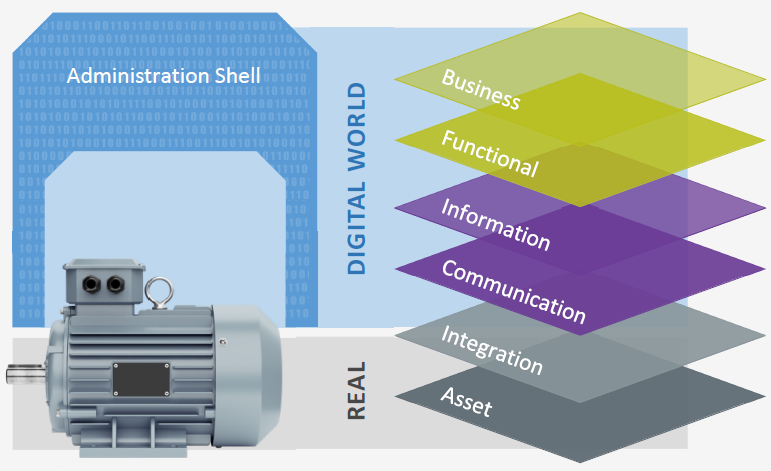
\includegraphics[width=1\textwidth]{aas-rami.png}
		\label{fig:aas-rami}
		\source{\citeonline{germany2018ramistandardization} (adaptado).}
	\end{figure}
		
	O AAS consiste em vários submodelos nos quais são descritos todas as informações e funcionalidades de um determinado ativo, incluindo suas características, propriedades, condição, parâmetros, dados de medições e capacidades \cite{bader2019aas}. A Figura \ref{fig:aas-submodelos} exemplifica um AAS como sendo uma ``casca'' que engloba o ativo em si, essa casca contém informações relevantes do ativo em forma de ``submodelos''.
	
	\begin{figure}[H]
		\centering
		\caption{Exemplificação de um AAS para um servomotor, incluindo os submodelos de dados técnicos, dados operacionais e documentação.}
		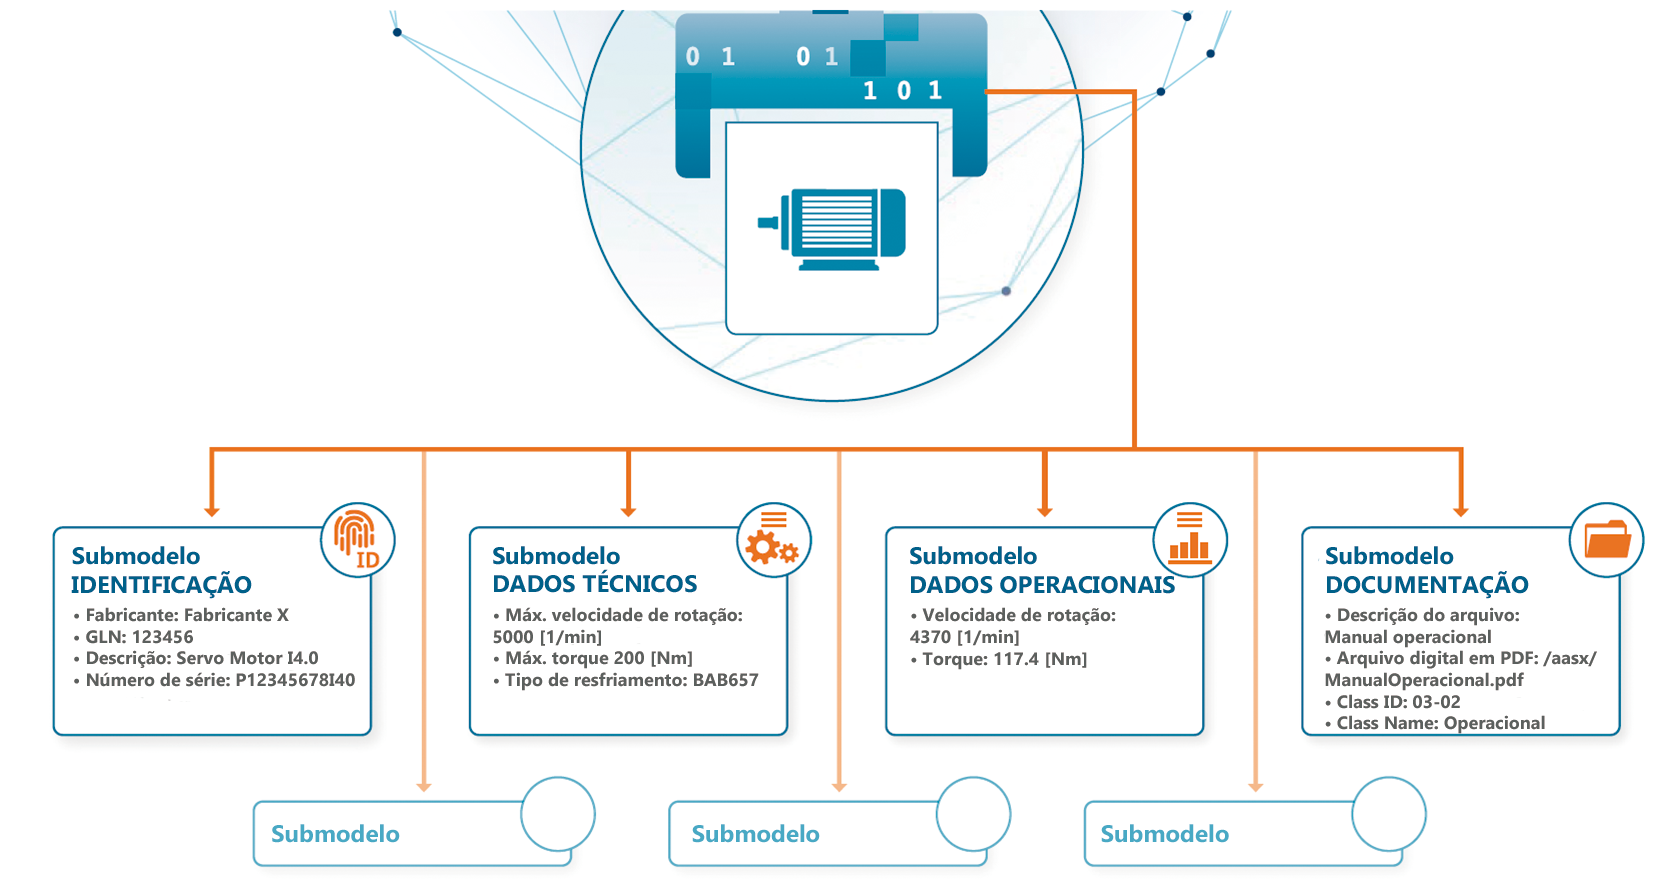
\includegraphics[width=1\textwidth]{aas-submodelos.png}
		\label{fig:aas-submodelos}
		\source{\citeonline{zvei2019aas} (adaptado).}
	\end{figure}
	
	O ASS permite o uso de diferentes canais de comunicação entre objetos na I4.0, é um elo entre os objetos físicos e o mundo conectado. A Figura \ref{fig:aas-conexao} ilustra a comunicação entre diferentes AASs em um ambiente de manufatura I4.0.
	
	\begin{figure}[H]
		\centering
		\caption{Comunicação entre AAS de objetos I4.0.}
		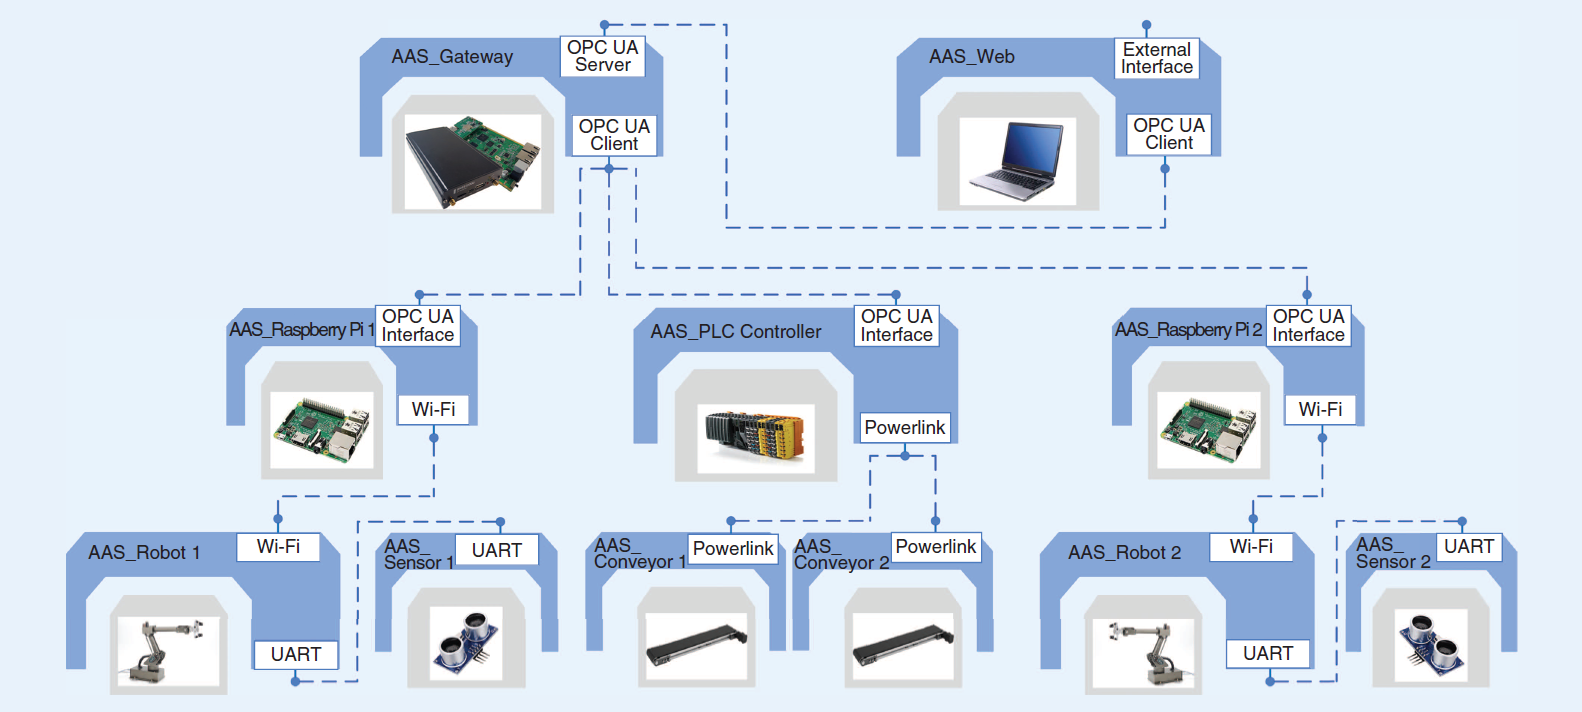
\includegraphics[width=1\textwidth]{aas-conexao.png}
		\label{fig:aas-conexao}
		\source{\citeonline{ye2019aas} (adaptado).}
	\end{figure}

	Dentro da I4.0, todos os ativos possuem um AAS com capacidade de comunicação com outros dispositivos. O conjunto Ativo-AAS, que é o objeto físico encapsulado pelo \textit{Administration Shell}, é denominado ``Componente I4.0''.
	
	A integração dos ativos, representados pelos Componentes I4.0, em um nível funcional requer uma descrição padronizada das funções (ou capacidades) dos ativos em questão. A padronização de submodelos para descrever detalhadamente cada função pode ser usada para definir requisitos para a fabricação de produtos \cite{bedenbender2017aasexamples}. A Figura \ref{fig:submodelos} mostra um exemplo de detalhamento de função do ativo.
	
	\begin{figure}[H]
		\centering
		\caption{Exemplo de detalhamento de função no AAS por meio de submodelos.}
		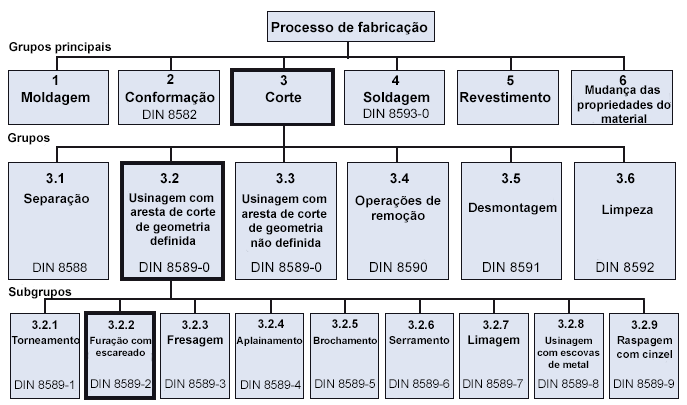
\includegraphics[width=1\textwidth]{submodelos.png}
		\label{fig:submodelos}
		\source{\citeonline{bedenbender2017aasexamples} (adaptado).}
	\end{figure}

	No ambiente de manufatura baseado na I4.0, o produto descreve os requerimentos necessários para sua fabricação e então esses requerimentos são comparados com as descrições da funções das máquinas disponíveis. Portanto, a seleção de um ativo é otimizada, baseando-se nos requerimentos do produto e nas descrições das funções dos ativos.
	

	\section{Memória digital do produto}

	Os produtos que são produzidos no cenário de Indústria 4.0 são equipados com a mémoria digital do produto (MDP). Por meio dessa memória podem ser acessadas e redistribuídas informações sobre o produto ao longo de toda a cadeia de valores.

	A MDP é alimentada e disponibilizada ao longo de todo o ciclo de vida do produto, podendo ser acessada por qualquer elo na cadeia de suprimentos (fabricante, distribuidor, varejista, consumidor). Mesmo no pós-venda a MDP ainda se faz presente. O consumidor ainda pode ter acesso às informações dos produtos em cada ponto da cadeia de suprimentos e se beneficiar de serviços individuais que se acumulam na memória \cite{brandherm2011productmemory}.

	Nesse contexto, a MDP mantém informações relevantes de eventos ocorridos ao longo do ciclo de vida do produto a fim de fornecer serviços a todo o ambiente com o qual o produto se relaciona \cite{brandherm2011productmemory}.
	
	A MDP fornece também uma forma de rastreabilidade de produtos ao longo da cadeia de valores uma vez que pode armazenar informações geoespaciais do ativo ao longo do tempo.



% ----------------------------------------------------------
\chapter{Inserção de MDP no RAMI4.0}

	O conceito de Memória Digital do Produto (MDP) é inserido dentro da Indústria 4.0 com o objetivo de se agregar valor por meio da possibilidade de compartilhamento de informações entre parceiros ao longo da cadeia de valor de um ativo através da Internet.
	
	A MDP é definida neste trabalho como um submodelo do AAS de um ativo qualquer. O submodelo MDP é composto de dados e funções de processamento de dados.
	
	O submodelo MDP não armazena dados, ficando a cargo de cada submodelo o armazenamento de dados referente ao seu próprio escopo de interesse. O MDP, entretanto, agrega os dados de diferentes submodelos por meio de \textit{links} com a base de dados de todos os demais submodelos. O MDP é uma forma de integração dos dados feita por meio do espelhamento dos dados de submodelos diversos na forma de somente leitura (\textit{read-only}). A Figura \ref{fig:submodeloMDP} ilusta funcionamento do acesso aos dados por parte do submodelo MDP.
	
	\begin{figure}[H]
		\centering
		\caption{.}
		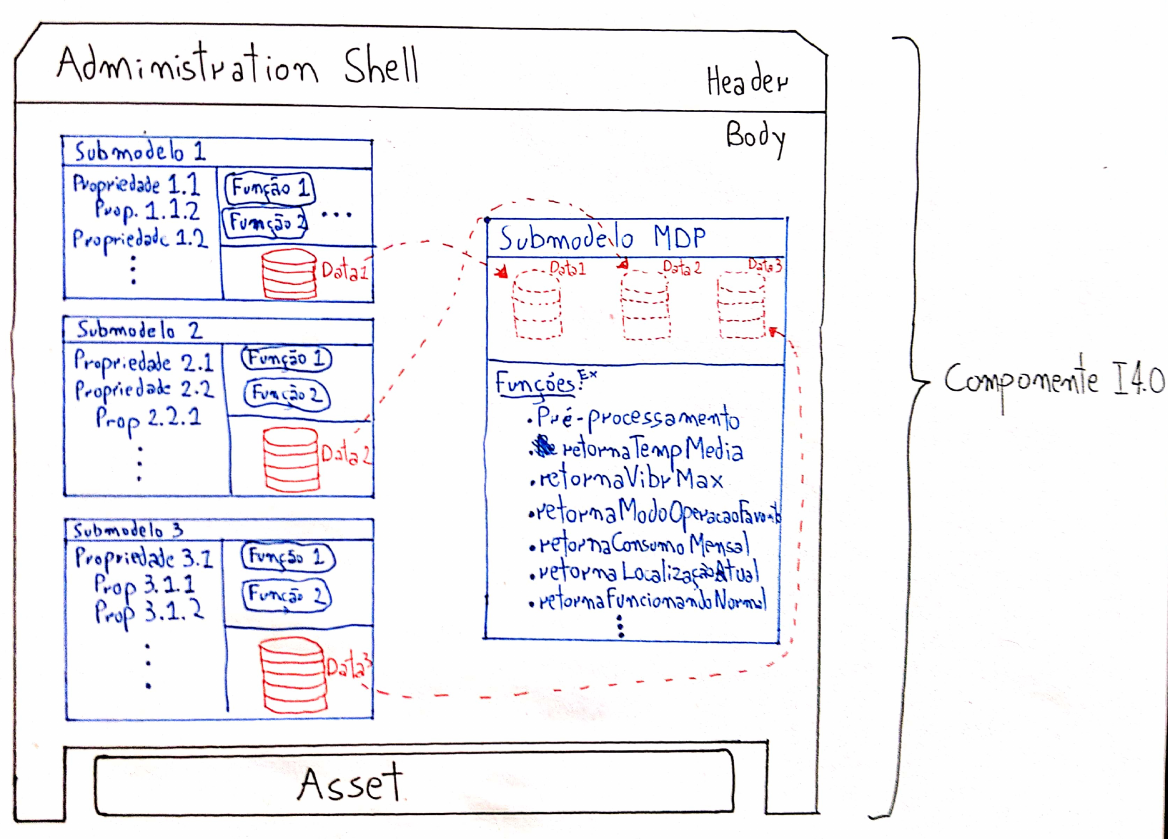
\includegraphics[width=1\textwidth]{submodeloMDP.png}
		\label{fig:submodeloMDP}
		\source{O autor.}
	\end{figure}`

	A comunicação entre o submodelo MDP e os demais modelos é essencial, pois o MDP depende da acessibilidade da base de dados dos demais submodelos para o processamento de suas funções. 
	
	

% ----------------------------------------------------------
\chapter{Publicações decorrentes do trabalho}

	\textbf{Publicação 1}:
	\begin{itemize}
		\item \underline{Título do trabalho}: “Análise de implementação de IoT na cadeia logística”
		\item \underline{Congresso}: XXXIX Encontro Nacional de Engenharia de Produção - ENEGEP 2019
		\item \underline{Status}: Aprovado, apresentado e publicado nos anais do evento
		\item \underline{Autores}:  Henrique A. Vitoi, Fabrício Junqueira, Paulo E. Miyagi
		\item \underline{Apresentação}: 16 de outubro de 2019, Santos/SP
	\end{itemize}
	
	\bigskip
	

	\textbf{Publicação 2}:
	\begin{itemize}
		\item \underline{Título do trabalho}: “Big Data on Machine to Machine Integration's Requirement Analysis Within Industry 4.0”
		\item \underline{Congresso}: DoCEIS 2019: Technological Innovation for Industry and Service Systems
		\item \underline{Status}: Aprovado e publicado
		\item \underline{Autores}:  Felipe A. Coda, Rafael M. Salles, Henrique A. Vitoi, Marcosiris A. O. Pessoa, Lucas A. Moscato, Diolino J. Santos Filho, Fabrício Junqueira, Paulo E. Miyagi
		\item \underline{Publicação}: 16 de abril de 2019
	\end{itemize}




% ----------------------------------------------------------
\chapter{Cronograma detalhado}

	O cronograma planejado é mostrado na Tabela \ref{tab:cronograma}.
	
	\begin{table}[H]
		\centering
		\caption{Cronograma detalhado de atividades}
		\makebox[\textwidth][c]{\footnotesize
		\begin{tabular}{|c|c|c|c|c|c|c|c|c|c|c|c|c|}
			
			\hline 
			
			& \multicolumn{2}{c|}{2018}
			& \multicolumn{6}{c|}{2019}
			& \multicolumn{4}{c|}{2020} \\
			
			\hline
			Etapas
			& \begin{tabular}[c]{@{}c@{}}set/\\   out\end{tabular} 
			& \begin{tabular}[c]{@{}c@{}}nov/\\   dez\end{tabular} 
			& \begin{tabular}[c]{@{}c@{}}jan/\\   fev\end{tabular} 
			& \begin{tabular}[c]{@{}c@{}}mar/\\   abr\end{tabular} 
			& \begin{tabular}[c]{@{}c@{}}mai/\\   jun\end{tabular} 
			& \begin{tabular}[c]{@{}c@{}}jul/\\   ago\end{tabular} 
			& \begin{tabular}[c]{@{}c@{}}set/\\   out\end{tabular} 
			& \begin{tabular}[c]{@{}c@{}}nov/\\   dez\end{tabular} 
			& \begin{tabular}[c]{@{}c@{}}jan/\\   fev\end{tabular} 
			& \begin{tabular}[c]{@{}c@{}}mar/\\   abr\end{tabular} 
			& \begin{tabular}[c]{@{}c@{}}mai/\\   jun\end{tabular}
			& \begin{tabular}[c]{@{}c@{}}jul/\\   ago\end{tabular} \\ 
			
			\hline
			Cumprimento dos créditos 
			& \cellcolor[HTML]{9AFF99}C
			& \cellcolor[HTML]{9AFF99}C 
			& \cellcolor[HTML]{9AFF99}C 
			& \cellcolor[HTML]{9AFF99}C 
			& \cellcolor[HTML]{9AFF99}C 
			& \cellcolor[HTML]{9AFF99}C 
			&
			&
			&
			&
			& \\
			
			\hline
			Levantamento bibliográfico
			& \cellcolor[HTML]{9AFF99}C
			& \cellcolor[HTML]{9AFF99}C
			& \cellcolor[HTML]{9AFF99}C
			& \cellcolor[HTML]{9AFF99}C
			& \cellcolor[HTML]{9AFF99}C
			& \cellcolor[HTML]{9AFF99}C
			& \cellcolor[HTML]{9AFF99}C
			& \cellcolor[HTML]{9AFF99}C
			& \cellcolor[HTML]{FFCB2F}A
			& \cellcolor[HTML]{FFCB2F}A
			& \cellcolor[HTML]{FFCB2F}A
			& \cellcolor[HTML]{FFCB2F}A \\
			
			\hline
			Desenvolvimento do projeto
			&
			&
			& \cellcolor[HTML]{9AFF99}C
			& \cellcolor[HTML]{9AFF99}C
			& \cellcolor[HTML]{9AFF99}C
			& \cellcolor[HTML]{9AFF99}C
			& \cellcolor[HTML]{9AFF99}C
			& \cellcolor[HTML]{9AFF99}C
			& \cellcolor[HTML]{FFCB2F}A
			& \cellcolor[HTML]{FFCB2F}A
			& \cellcolor[HTML]{FFCB2F}A
			& \\ 
			
			\hline
			Exame de Qualificação
			&
			&
			&
			&
			&
			&
			&
			&
			&
			& \cellcolor[HTML]{FFCB2F}A
			&
			& \\
			
			\hline
			Defesa da dissertação
			&
			&
			&
			&
			&
			&
			&
			&
			&
			&
			&
			& \cellcolor[HTML]{FFCB2F}A \\
			\hline
			
		\end{tabular}}
		\label{tab:cronograma}
		\source{O autor.}
	\end{table}

	A data estipulada para defesa da dissertação pode ser adiada conforme necessidade para refinamento do projeto, adicionando-se mais meses para levantamento bibliográfico e desenvolvimento do projeto, respeitando de toda forma o prazo máximo para depósito da dissertação. 
	
	Disciplinas cursadas nos períodos 2018/3, 2019/1 e 2019/2:
	\begin{itemize}
		\item PMR5024 - Simulação de Sistemas;
		\item PTC5751 - Internet das coisas;
		\item PEA5003 - Sistemas Inteligentes de Transporte;
		\item PMR5023 - Modelagem e Análise de Sistemas;
		\item PTR5744 - Pesquisa Operacional;
		\item PRO5807 - Logística e Cadeia de Suprimentos;
		\item PMR5402 - Controle de Sistemas.
	\end{itemize}

	% Dizer no que as disciplinas ajudaram no trabalho. 
	


% ----------------------------------------------------------
\chapter{Conclusão}
	\lipsum[1-1]
	
	\cite{aruvali2014objectmemory}
	\cite{toro2015intelligentsystems}
	\cite{vaidya2018industryfour}
	\cite{souit2013soa}
	.














% ----------------------------------------------------------
% ELEMENTOS PÓS-TEXTUAIS
% ----------------------------------------------------------
\postextual
\bibliography{ref}

\end{document}
